% Project:			Mediation and Gender Differences
% This file:		Main writeup
% Original date: 	December 7, 2016

\documentclass[11pt]{article}

% colors
\usepackage[table]{xcolor}
\definecolor{maroon}{RGB}{153,0,18}
\definecolor{lime}{RGB}{190,213,88}
\definecolor{sand}{RGB}{217,202,179}
\definecolor{fire}{RGB}{144,50,61}
\definecolor{brick}{RGB}{94,11,21}
\definecolor{olive}{RGB}{117,109,84}
\definecolor{lavpink}{RGB}{172,123,132}
\definecolor{darkpurp}{RGB}{49,10,49}
\definecolor{salmon}{RGB}{204,90,113}
\definecolor{mauve}{RGB}{94,73,85}
\definecolor{greyblue}{RGB}{125,132,145}
\definecolor{greypurp}{RGB}{68,56,80}
\definecolor{brightpurp}{RGB}{96,20,255}

% packages (please add in alphabetical order)
\usepackage{adjustbox}
\usepackage{amsfonts}
\usepackage{amsmath}
\usepackage{amssymb}
\usepackage{array}
\usepackage{bm}
\usepackage{booktabs}
\usepackage{caption}
\usepackage{epstopdf}
\usepackage{float}
\usepackage[margin=1in]{geometry}
\usepackage{graphicx}
\usepackage[colorlinks=true, linkcolor=brightpurp, citecolor=brightpurp, urlcolor=salmon]{hyperref}
\usepackage{lipsum}
\usepackage{longtable}
\usepackage{mathtools}
\usepackage{multirow}
\usepackage{natbib}
\usepackage{rotating}
\usepackage{setspace}
\usepackage{subcaption}
%\usepackage{threeparttable}
\usepackage{threeparttablex}
\usepackage{xr}
\usepackage[printwatermark]{xwatermark}


\newcolumntype{L}[1]{>{\raggedright\let\newline\\\arraybackslash\hspace{0pt}}m{#1}}
\newcolumntype{C}[1]{>{\centering\let\newline\\\arraybackslash\hspace{0pt}}m{#1}}
\newcolumntype{R}[1]{>{\raggedleft\let\newline\\\arraybackslash\hspace{0pt}}m{#1}}

% commands
\newcommand{\mr}{\multirow}
\newcommand{\mc}{\multicolumn}

%Other parameters
\newcommand{\noutcomes}{95}
\newcommand{\treatsubsabc}{$75\%$}
\newcommand{\treatsubscarec}{$74\%$}
\newcommand{\treatsubscaref}{$63\%$}

%Counts
%Males
\newcommand{\positivem}{$79\%$}
\newcommand{\positivesm}{$37\%$}

%Females
\newcommand{\positivef}{$73\%$}
\newcommand{\positivesf}{$35\%$}

%Counts, control substitution
%Males
\newcommand{\positivecsnm}{$58\%$}
\newcommand{\positivescsnm}{$25\%$}

\newcommand{\positivecsam}{$74\%$}
\newcommand{\positivescsam}{$38\%$}

%Females
%% no alternative
\newcommand{\positivecsnf}{$83\%$}
\newcommand{\positivescsnf}{$46\%$}

%% alternative
\newcommand{\positivecsaf}{$73\%$}
\newcommand{\positivescsaf}{$23\%$}

%Pooled

%Effects
%Males

%Females
\newcommand{\hsgradf}{$7$}
\newcommand{\yearsedf}{$1.2$}



%Pooled

%CBA
%IRR
%Males
\newcommand{\irrm}{$15\%$}
\newcommand{\irrsem}{$13\%$}

%Females
\newcommand{\irrf}{$10\%$}
\newcommand{\irrsef}{$12\%$}

%Pooled
\newcommand{\irrp}{$13\%$}
\newcommand{\irrsep}{$11\%$}

%BC
%Males
\newcommand{\bcm}{$7.88$}
\newcommand{\bcsem}{$8.06$}

%Females
\newcommand{\bcf}{$2.30$}
\newcommand{\bcsef}{$1.56$}

%Pooled
\newcommand{\bcp}{$4.35$}
\newcommand{\bcsep}{$2.57$}

%NPV streams
%Pooled
\newcommand{\parincomenpvp}{$\$115,026$}

\externaldocument{treatmenteffects_appendix}

\begin{document}


\title{Gender Differences in the Benefits of an Early Childhood Program}
\author{Jorge Luis Garc\'{i}a \and James J. Heckman \and Anna L. Ziff}
\date{Original date: December 7, 2016 \\ Current date: \today}
\maketitle

\section{Outline}

\begin{enumerate}
\item	Introduction
	\begin{enumerate}
		\item There are gender differences in the current economy. These are especially pronounced when considering disadvantage as well.
		\item These differences can arise early in life (show plots with gender differences of skills)
		\item Differences can propagate over the life cycle (show plots with adult gender differences)
		\item This paper studies the effects of ABC/CARE and offers two methodological innovations (combining functions, counterfactual) to show stark gender differences
		\item Summary of main findings
		\item We offer an explanation of the differences (summarize mechanism)
		\item Paragraph of related literature
		\item Roadmap
	\end{enumerate}
\item Program
	\begin{enumerate}
		\item Description of ABC/CARE intervention and study
		\item Description of data collection points and measures collected
	\end{enumerate}
\item Parameters of interest
\item Combining functions
\item Results
	\begin{enumerate}
		\item Plots of combining functions
		\item Treatment effects mostly presented in the appendix
	\end{enumerate}
\item Mediation
	\begin{enumerate}
		\item Description of mechanism
	\end{enumerate}
\item Conclusion
\end{enumerate}

\noindent This paper studies the life-cycle impacts of a high-quality, intensive, influential, and widely emulated early childhood program that started early in life (at 8 weeks of age) and had a randomized design. Upon the impracticality of analyzing the dozens of outcomes available to evaluate the program one at the time and the need to avoid cherry-picking outcomes with significant treatment effects, we propose parametric and non-parametric tests to aggregate and summarize treatment effects. We document that girls benefit more than boys. The source of this difference is a worst counterfactual to treatment for girls which results from baseline socio-economic disadvantage. \textbf{[Word count: 100 words.]}

\tableofcontents

\doublespacing

\section{Introduction}
\label{sec:introduction}


This paper studies two influential early childhood programs offered as an educational form of childcare. The programs are the Carolina Abecedarian Project (ABC) and its almost identical sister program, the Carolina Approach to Responsive Education (CARE), both evaluated by the method of random assignment---henceforth ABC/CARE. While certain features and categories of outcomes of ABC/CARE have been thoroughly assessed, our paper is the first to aggregate and summarize all of the available outcomes to evaluate the program, including, for example, adulthood administrative criminal records.

ABC/CARE was conducted in Chapel Hill, North Carolina for a sample of children born between 1972 and 1980. It was one of the pioneer programs that focused intensively on child-led learning and is a template for many current and proposed early childhood programs.\footnote{Programs inspired by ABC/CARE have been (and are currently being) launched around the world. \citet{Sparling_2010_Highlights} and \citet{Ramey_Ramey_Lanzi_2014_Interventions} list numerous programs based on the ABC/CARE approach. The programs are: IHDP---eight different cities around the U.S. \citep{Spiker-etal_1997_Helping}; Early Head Start and Head Start in the U.S. \citep{Schneider_McDonald-eds_2007_Scale-Up_Vol-1}; John's Hopkins Cerebral Palsy Study in the U.S. \citep{Sparling_2010_Highlights}; Classroom Literacy Interventions and Outcomes (CLIO) study in the U.S. \citep{Sparling_2010_Highlights}; Massachusetts Family Child Care Study \citep{Collins_etal_2010_Massachusetts-Study}; Healthy Child Manitoba Evaluation \citep{Healthy_Child_Manitoba_2015_Starting-Early}; Abecedarian Approach within an Innovative Implementation Framework \citep{Jensen_Nielsen_2016_ABC-Programme-Pilot}; and Building a Bridge into Preschool in Remote Northern Territory Communities in Australia \citep{UMonash_Dataset_2015_URL}. Educare programs are also based on ABC/CARE \citep{Educare_2014_Research_Agenda,Yazejian_Bryant_2012_Educare}.} It started at 8 weeks of age and continued through age 5. Treatment and control children were followed through their mid 30s, with data collected on multiple dimensions of human development. As a result of this intensive data collection, there are over 100 outcomes that we could use to evaluate the program.

Given the difficulty of individually analyzing the hundreds of available outcomes to evaluate the program and the need to avoid cherry-picking outcomes with significant treatment effects, we propose parametric and non-parametric tests to aggregate and summarize treatment effects. Table~\ref{table:summary} previews our approach. Panel (a) displays our summaries for early-childhood outcomes (birth to age 5). We offer four treatment-control comparisons across these outcomes by gender: (i) the average effect size; (i) the percentage of outcomes for which there is a positive treatment effect; (iii) the percentage of outcomes for which there is a positive and significant ($\alpha=10\%$) effect; and (iv) the asymptotic approximation of the $p$-value resulting from a non-parametric comparison of the joint distribution of outcomes \citep{Rosenbaum_2005_Distribution_JRSS}. Panels (b) and (c) are analogous for school age (ages 6 to 18) and adulthood (21 to 35), respectively, and Panel (d) includes all of the outcomes in Panels (a) through (c).


\begin{table}[!htpb]
\begin{threeparttable}
\caption{Summary of Treatment-Control Comparisons by Gender} \label{table:summary}
\centering 
\begin{tabularx}{16.5cm}{XcX}
& 

\begin{tabular}{lcccc} 
\toprule
 & \mc{2}{c}{\textbf{(a) Childhood}}   & \mc{2}{c}{\textbf{(b) School Age}}  \\
 & Females & Males & Females & Males \\
 \cmidrule(lr){2-3}  \cmidrule(lr){4-5}
 Average Effect Size &      \textbf{    0.367} &    \textbf{    0.316} &     \textbf{    0.395} &     0.214 \\  
 \% $>0$ Treatment Effect &    \textbf{   95.833}  &     \textbf{   75.000}	&	 \textbf{  100.000} &   \textbf{  100.000}  \\  
 \% $>0$, Significant Treatment Effect&     \textbf{   62.500}  &   \textbf{   37.500} &    \textbf{   55.556} &     \textbf{   44.444} \\  
\citet{Rosenbaum_2005_Distribution_JRSS} $p$-value &     \textbf{0.086} &     \textbf{0.086} 	&       \textbf{0.022} &     0.147 \\  
 \midrule
 & \mc{2}{c}{\textbf{(c) Adulthood}}   & \mc{2}{c}{\textbf{(d) All}}  \\
 & Females & Males & Females & Males \\
  \cmidrule(lr){2-3}  \cmidrule(lr){4-5}
 Average Effect Size  &     \textbf{    0.298} &    \textbf{    0.399} &     \textbf{    0.348} &  \textbf{0.327} \\  
 \% $>0$ Treatment Effect  &    \textbf{   88.889} &    \textbf{   72.222} & \textbf{   94.118} &    \textbf{   78.431} \\  
 \% $>0$, Significant Treatment Effect &    \textbf{   50.000}  &    \textbf{   33.333}	&    \textbf{   56.863}&    \textbf{   37.255} \\  
\citet{Rosenbaum_2005_Distribution_JRSS} $p$-value &     \textbf{0.010} &     \textbf{0.086} 	&       \textbf{0.010} &     \textbf{0.086} \\  
\bottomrule
\end{tabular}


% This table displays summaries of treatment effects by age and gender. Each of the panels contains statistics calculated using outcomes measured at the indicated ages. Early childhood includes outcomes measured before age 6, school age includes outcomes measured between age 6 and 18, and adult includes outcomes measured after 18. All (panel d), is a combination of all the outcomes in panels a-c. The average effect size is calculated by averaging over the effect size of the outcomes in the age category. The effect sizes of the individual outcomes are calculated by dividing the coefficient by the standard deviation of the control group. The $p$-values are asymptotic following \citet{Rosenbaum_2005_Distribution_JRSS}. The null hypothesis is that the control and treatment distributions, within gender, are equal. A $p$-value less than 0.1 indicates that the distributions are significantly different.  & 
\end{tabularx}
\begin{tablenotes}
\footnotesize
\item \textbf{Note:} This table displays summaries of treatment effects by age and gender. Each of the panels contains statistics calculated using outcomes measured at the indicated ages. Early childhood includes outcomes measured before age 6, school age includes outcomes measured between age 6 and 18, and adult includes outcomes measured after 18. All (panel d), is a combination of all the outcomes in panels (a) to (c). The average effect size is calculated by averaging over the effect size of the outcomes in the age category. The effect sizes of the individual outcomes are calculated by dividing the coefficient by the standard deviation of the control group. The \citet{Rosenbaum_2005_Distribution_JRSS} $p$-value originates from a test where the null is a common joint distribution of the variables in each category. A $p$-value less than $0.10$ (bolded) indicates that the distributions are significantly different at the 10\% level. More details on our inference procedure are in Section~\ref{sec:parameters}.
\end{tablenotes}
\end{threeparttable}
\end{table}

The first finding in Table~\ref{table:summary} is that randomized assignment to ABC/CARE benefited both females and males across the life cycle. Across the life-cycle, the average effect size for females (males) is $0.381$ ($0.254)$, the percentage of positive treatment effects is $94\%$ ($78\%$), and the percentage of significant treatment effects at the $10\%$ level is $43\%$ ($22\%$). Standard inference could be provided for these three measures. Instead, we provide the $p$-value of a non-parametric test contrasting the joint distribution of the outcomes. The conclusion from these comparisons aligns with the conclusions from the other measures, even in magnitude if the size of the $p$-value is taken as a measure of magnitude \citep{Fisher_1935_Inference_JRSS}. A disadvantage of our summaries is the loss of perspective on the magnitudes of the effects, which we describe and discuss further below.\footnote{For example, assignment to treatment increased college graduation for males by 17 percentage points, with a standard error of 5 percentage points and where the college graduation rate for the control group is 12\%. For females, assignment to treatment increased high school graduation by 25 percentage points, with a standard error of 1 percentage point and where the high school graduation rate for the control group is 53\% points. These results are the basis of the forecasts in \citet{Garcia_Heckman_Leaf_etal_2017_Comp_CBA_Unpublished}: The authors document that education is actually the main intermediate input when forecasting benefits across the life cycle.}

The second finding in Table~\ref{table:summary} is that females benefit more than males. This holds across the life cycle and across all of the measures that we employ to summarize the treatment effects. To explain the gendered treatment effects, we document that control-group girls grew up in a less favorable environment if compared to control-group boys using baseline measures (e.g.,\ less father presence, lower maternal education and IQ). Girls in the control group who stayed at home ($23\%$ of the control-group girls), were taken care of in a disadvantaged environment. Girls who went to preschools other than ABC/CARE ($77\%$ of the control-group girls), likely went to the lowest quality preschools because their families were more resource constrained if compared to their boy counterparts. Thus, girls benefited more from treatment because they would have otherwise grown up in a relatively worst environment if compared to boys.\footnote{Documentation in \citet{Burchinal_etal_1989_CD_Daycare-Pre-K-Dev} shows that the quality of the available alternatives was of lower quality than the treatment offered through ABC/CARE. We supplement this documentation with historical records showing that even the alternatives that followed state and federal standards of the era, were of lower quality than ABC/CARE as measured by concrete measures such as staff-child ratios. We provide more detail on the quality of ABC/CARE and the alternative options in Section~\ref{sec:data} and Appendix~\ref{appendix:background}.}

Although there was no significant difference in the take-up of preschool alternatives between control-group parents of girls and control-group parents of boys, there is a subtle, important difference in the within-gender take-up of alternatives. Within girls, take-up of alternatives does not differ significantly by socio-economic disadvantage, although we show later that more disadvantaged control-group parents of girls select home care. Within boys, the relatively advantaged stayed at home more often and did not attend the relatively low-quality preschool alternatives available in the area at the time when ABC/CARE was implemented. These results are verified when we estimate parameters that explicitly account for control substitution. That is, when we compare treatment to alternative preschools and treatment to staying at home. These parameters are not identified by randomization into treatment and require the stronger assumptions that we discuss below. Boys benefit the most from ABC/CARE when compared to alternative preschools, given their relatively better home environment. Girls benefit the most from ABC/CARE when compared to home environments, given that those who stay at home are more disadvantaged. The difference in this benefit is less than the difference for boys, which is consistent with the stronger presence of selection for boys.

ABC/CARE greatly benefits children by providing an enriching environment to complement their home environments. This sounds a cautionary note for advocates of early childhood programs in any form: Quality matters and low-quality programs could cause harm. Dissecting the counterfactual brings our results to a modern context in which many children are enrolled in preschool, and in which low-quality is abundant for children from socio-economic disadvantaged backgrounds.\footnote{Approximately 60\% of preschool-age children regularly receive non-parental childcare \citep{FIFCFS_2009_Wellbeing_REPORT}. At age 4, the child care break down for disadvantaged children, which compose 13\% of all children in the US \citep{USCB_2014_CoverageReport}, was the following. Head Start: 29\%; Non-Head Start center-based: 26\%; relative care: 15\%; non-relative care: 5\%; parental care: 25\%. While the quality of Head Start centers and family day care arrangements is constant across poor and non-poor children, the quality of the rest of arrangements is considerably and consistently lower for poor children, when compared to non-poor children. This according to Early Childhood Environment and family Dat Care scaled \citep{FIFCFS_2009_Wellbeing_REPORT}.}

The rest of our analysis unfolds in the following way. Section~\ref{sec:data} describes the experimental data we analyze and its special features. It documents the quality level of the alternative childcare that a considerable proportion of the control-group subjects attended. Section~\ref{sec:parameters} defines the treatment effects we estimate and how we summarize them. Section~\ref{sec:treatment-effects} reports the treatment effects overall and by gender and establishes the existence of sharp gender differences for many categories of outcomes. Section~\ref{sec:gender-differences} discusses the sources of these differences. Section~\ref{sec:conclusion} concludes.
	

\section{Background and Data}
\label{sec:data}
We analyze a combined sample of the two closely related programs, ABC and CARE. Table~\ref{tab:abc-care-characteristics} summarizes their characteristics. Both interventions were implemented by researchers at the Frank Porter Graham Center (FPG) at the University of North Carolina Chapel Hill, and targeted children from disadvantaged families in the Chapel Hill area. ABC had four cohorts born between 1972 and 1977, and CARE had two cohorts born between 1978 and 1980. Eligibility was determined on the basis of the High Risk Index (HRI) developed for ABC and adapted for CARE \citep{Campbell_Wasik_etal_2008_ECRQ}. Components of the HRI include father's presence, parental employment, and participation in welfare.\footnote{See Appendix~\ref{app:eligibility-pop} for the full list of the determinants of HRI \citep{Ramey_Smith_1977_AJMD, Wasik_Ramey_etal_1990_CD, Ramey_Campbell_1991_childreninpoverty}.} Based on these eligibility requirements, \citet{Garcia_Heckman_Leaf_etal_2017_Comp_CBA_Unpublished} calculate that 43\% of all African American children would be eligible now and that 19\% were eligible during the intervention.

Both interventions involved free, intensive center-based care for subjects in the treatment group starting at 8 weeks and continuing until age 5 before the children started kindergarten. Treatment-group subjects also received daily health screenings, diapers, and formula until 6 months. Control-group families received diapers and formula as well for the same period of time \citep{Wasik_Ramey_etal_1990_CD,Ramey_Campbell_1991_childreninpoverty}. Between ages 5 and 8, there was an additional component of treatment in which home visitors worked with children and their parents to tutor the children and to encourage families to be involved in their child's schooling. In CARE, all the subjects who received center-based care also received this school-age component. In ABC, treatment status of this component was randomized. We do not analyze this part of the treatment because previous work has found this component of the treatment to have no significant effects \citep{Campbell_Ramey_etal_2002_ADS,Campbell_Conti_etal_2014_EarlyChildhoodInvestments}.

\begin{table}[!htbp]
\centering
\caption{Overview of the ABC and CARE Programs}
\label{tab:abc-care-characteristics}
\begin{threeparttable}
	\begin{tabular}{l l}
	\toprule
Site & Chapel Hill, North Carolina \\
Cohorts & 4 (ABC), 2 (CARE) \\
$N$ & 58 treatment, 56 control (ABC) \\
	& 17 treatment, 23 control (CARE) \\
\midrule
Eligibility & HRI $>$ 11 \\
		& Biologically healthy \\
\midrule
Treatment years & 1972--1981 (ABC), 1977--1985 (CARE) \\
Treatment duration & 5 years \\
\midrule
Home visits 	& 2.5--2.7	per month (CARE)	\\
Center care	& 50	weeks per year \\
		 	& 30--45 hours per week  \\
Other treatment components & Formula until 6 months\\
					& Diapers until 6 months \\ 
					& Health check-ups \\
					& Medical care \\
					& Parenting instruction \\
					& Counseling \\
					& Transportation to center \\
Control-group incentives & Formula until 6 months \\
				& Diapers until 6 months 	\\
				& Health check-ups until 1 year (ABC, cohort 1) \\
\midrule
Adult-child ratio & 1:3--1:6 \\
Teacher requirements & High school through masters \\
				& Experience with kids \\
Specialists & Physician, nurse, social worker \\
\bottomrule
\end{tabular}



\begin{tablenotes}
\footnotesize
\item Note: Characteristics that do not specify ABC or CARE were present in both. Biologically healthy includes lack of serious illness, including mental retardation. HRI is the High Risk Index. This table is adapted from \citet{Elango_Hojman_etal_2016_Early-Edu}. \\
\item Sources: \citet{Ramey_Collier_etal_1976_CarolinaAbecedarianProject,Ramey_Smith_1977_AJMD,Ramey_etal_1985_Project-CARE_TiECSE,Wasik_Ramey_etal_1990_CD,Ramey_Campbell_1991_childreninpoverty}. 
\end{tablenotes}
\end{threeparttable}
\end{table}

The program focused on developing language, cognition, and social-emotional skills. During ABC and CARE, the \textit{Learning Games} curriculum was developed and refined \citep{Sparling_Lewis_1979_BOOKLearninggamesFirstThree}. Other curricula used in the program emphasized child-led learning of skills important for future learning \citep{Ramey_Smith_1977_AJMD, Wasik_Ramey_etal_1990_CD, Ramey_Campbell_1991_childreninpoverty}. The teachers and classroom aids were trained continuously throughout the intervention. Researchers and child development experts at FPG observed the classroom interactions and relayed detailed feedback to the instructors \citep{Ramey-etal_2012-ABC}.

These aspects of the program relate to structural quality rather than process quality, i.e., the daily experiences of the children \citep{Thomason_LaParo_2009_EED}. Aspects of structural quality, including low child-teacher ratios, small group sizes, and teacher education, are often associated with high process quality \citep{Phillipsen_etal_1997_ECRQ}. However, recent studies find that curricula and professional development are even more highly correlated with process quality. This is especially true if the curricula and professional development are informed by knowledge of child development \citep{Slot_etal_2015_Dutch_ECRQ}. Although measures of process quality (e.g., measures of teacher-child interactions) are not available for the ABC/CARE subjects, the curricula and professional development offerings were exceedingly intensive, especially compared to standards of that era \citep{Ramey-etal_2012-ABC}. \textbf{[JJH: discussion off mark] [JLG: Yes, to me this is some real ed school bs, but referee 4 asks us to put this information in her ``minor'' comments 1.]}

CARE included an additional arm of treatment. Besides the services in Table~\ref{tab:abc-care-characteristics}, those in the treatment group also received home visiting from birth to age 5. Home visiting consisted of biweekly visits focusing on parental problem-solving skills. To individually test this home-visiting component, there was a third randomized group ($N=23$) that received only the home visiting component, but not center-based care \citep{Wasik_Ramey_etal_1990_CD}. In light of previous analyses finding no effect of this component, we drop this last group from our analysis.\footnote{\citet{Campbell_Conti_etal_2014_EarlyChildhoodInvestments} test and do not reject the hypothesis of no treatment effects for this additional component of CARE.} These analyses justify merging the treatment groups of ABC and CARE, even though that of CARE received the additional home-visiting component \citep{ABCCARE_Dataset}. We henceforth analyze the samples as coming from a single ABC/CARE program. This combination is also seen in \citet{Burchinal_etal_2006_MSRCD_IV-Growth-Curve}.

Table~\ref{tab:abccare-baseline} compares pre-program variables between experimental and gender groups. The only significant difference is seen in the HRI score, which is 1.78 points lower for males than for females. This indicates that males were slightly less advantaged at baseline. However, after accounting for multiple hypotheses using the Holm test, the difference in HRI score is no longer significant \citep{holm1979simple}.\footnote{For a more detailed description of the sample's disadvantage, see Appendix~\ref{app:eligibility-pop}.}

\begin{table}[!htbp]
\centering
\caption{Baseline Differences, ABC/CARE}
\label{tab:abccare-baseline}
\begin{threeparttable}
	\begin{tabular}{l c c c c c c}
\toprule
\mc{1}{c}{Variable} & Female & Male & $ p $ -value & Control & Treatment & $ p $ -value \\
& Mean & Differential & & Mean & Differential & \\
\midrule
Mother's age &                19.72 &                 1.13 &                 0.15 &                20.52 &                -0.51 &                 0.51 \\
Mother works &                 0.23 &                 0.09 &                 0.28 &                 0.21 &                 0.11 &                 0.18 \\
Mother's IQ &                84.46 &                 1.33 &                 0.46 &                84.65 &                 0.98 &                 0.58 \\
Father at home &                 0.24 &                 0.04 &                 0.56 &                 0.29 &                -0.05 &                 0.51 \\
Number of siblings &                 0.59 &                 0.07 &                 0.67 &                 0.71 &                -0.18 &                 0.29 \\
HRI score &                21.57 &                -1.78 &                 0.06 &                21.39 &                -1.47 &                 0.13 \\
Apgar score, 1 min. &                 7.68 &                -0.07 &                 0.80 &                 7.60 &                 0.09 &                 0.76 \\
Apgar score, 5 min. &                 8.94 &                -0.20 &                 0.33 &                 8.87 &                -0.04 &                 0.83 \\
Birthweight &                 7.18 &                -0.20 &                 0.34 &                 7.17 &                -0.19 &                 0.38 \\
Gestational age &                39.85 &                -0.42 &                 0.27 &                39.87 &                -0.50 &                 0.19 \\
\bottomrule
\end{tabular}
% This file generated by: /scripts/abccare/treatment-effects/abccare-baseline.do

\begin{tablenotes}
\footnotesize
\item Note: The variables in this table are all measured at the baseline age, close to when the children were born. A larger HRI (High Risk Index) score indicates more disadvantage. Apgar, measured at 1 and 5 minutes after birth, is a test of the health condition of newborn babies. A score closer to 10 indicates a healthier condition \citep{Apgar_1966_APGAR-Scoring_PCNA}. Birthweight is in pounds and gestational age is in weeks.
\end{tablenotes}
\end{threeparttable}
\end{table}

\indent \textbf{[JJH: Use Hold Test! Casual!] [JLG: Holm test in display now.]}


\subsection{The Randomization Protocol and its Compromises} \label{section:randomization}

Randomization for ABC/CARE was conducted on child pairs matched on family background. Siblings and twins were jointly randomized into either treatment or control groups. For siblings, this occurred when two siblings were close enough in age such that both of them were eligible for the program. Pairing was based on the High Risk Index, as well as maternal education, maternal age, and gender of the subject.\footnote{We do not know the original pairs.} 

ABC collected an initial sample of 121 subjects. All providers of health care and social services (referral agencies) in the area of the ABC/CARE study were informed of the programs. They referred mothers whom they considered disadvantaged. Eligibility was corroborated before randomization. Encouragement from the referral agencies was such that most referred mothers attended and agreed to participate in the initial randomization. We characterize each missing observation in Appendix~\ref{appendix:randomization}. In Appendix~\ref{appendix:estimates}, we document that our estimates are robust when we adjust for missing data using standard weighting (matching) methods described in Appendix~\ref{app:method_partialobs}. Twenty-two subjects in ABC did not stay in the program through age 5. The number of dropouts is evenly balanced across treatments and controls. Dropout was primarily related to the health of the child and the mobility of families rather than any dissatisfaction with the program. The 22 dropouts include four children who died, four children who left the study because their parents moved, and two children who were diagnosed as developmentally delayed. Details are in Table~\ref{table:abccompromises}. Everyone offered the program was randomized to either treatment or control. All eligible families agreed to participate. Dropping out occurs \emph{after} randomization and is balanced across treatment groups. We conduct the same analysis for the CARE sample, although there were far fewer dropouts and no compromised randomization.\footnote{The modest sample size, especially after dividing the sample by male and female, is unavoidable. No datasets have the experimental design and longitudinal data collection of ABC/CARE with a large sample. Future researchers should repeat these analyses in other, larger studies (e.g., the Infant Health and Development Program) as the subjects continue to age.} 

\subsection{Control Group Substitution}

In ABC/CARE, many control-group subjects (but no treatment-group subjects) attended alternative center-based care.\footnote{See \cite{Heckman_Hohmann_etal_2000_QJE} on the issue of substitution bias in social experiments.} The figure is \treatsubsabc\ for ABC and \treatsubscarec\ for CARE. This information is detailed in a survey administered to ABC/CARE families asking about the childcare arrangements made during each month between birth and age 5. Home care includes parental care, but also care of a relative, neighbor, or friend. The survey also captured specifics, such as the name of the center-based institutions, allowing for a more detailed understanding of the care environments.

\begin{sidewaysfigure}[!htbp]
\centering
\caption{Control Substitution Characteristics, ABC/CARE Control Group}\label{fig:control-sub}
\begin{subfigure}[h]{0.49\textwidth}
	\centering
	\caption{Cumulative Enrollment} \label{fig:treatsubcare}
	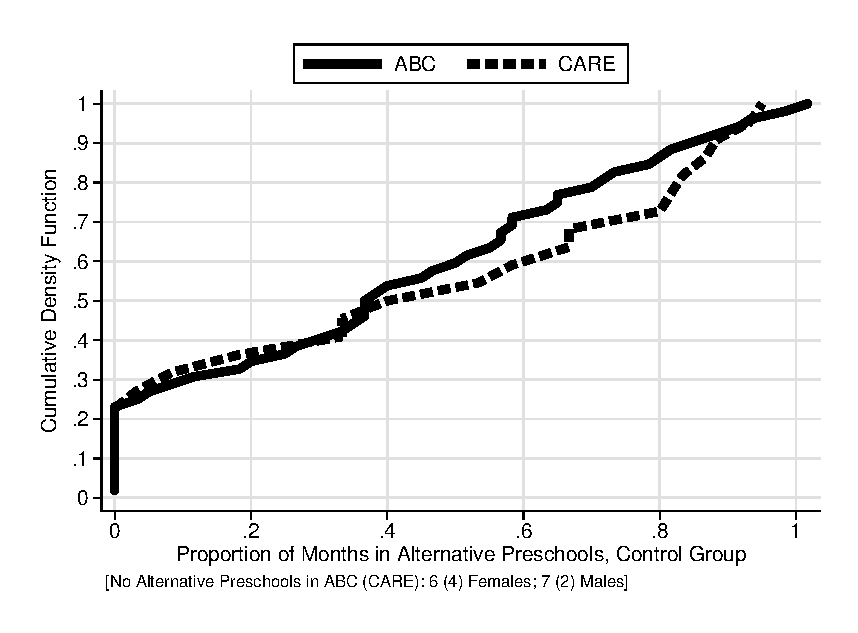
\includegraphics[width=\textwidth]{output/abccare_controlcontamination.eps}
\end{subfigure}
\begin{subfigure}[h]{0.49\textwidth}
	\centering
	\caption{Enrollment Dynamics} \label{fig:proportion-alt-pre}
	\includegraphics[width=\textwidth]{output/abccare_Vprobs.eps}
\end{subfigure}%
\footnotesize \justify
Note: Panel (a) displays the cumulative distribution function of enrollment in alternatives. Panel (b) displays the fraction of ABC/CARE control-group children enrolled in alternatives, conditional on being enrolled in the previous age (at least one month).\\
\end{sidewaysfigure}

Figure~\ref{fig:treatsubcare} shows the cumulative distribution of the proportion of time in the first five years that control subjects were enrolled in alternatives. Figure~\ref{fig:proportion-alt-pre} shows the dynamics of enrollment. Those who enroll generally stay enrolled. As control-group children aged, they were more likely to enter childcare (see Figure~\ref{fig:control-sub_a} in Appendix~\ref{app:control-subbb}).

Children in the control group enrolled in alternative early childcare programs are less economically disadvantaged at baseline compared to children who stay at home. Disadvantage is measured by maternal education, maternal IQ, Apgar scores, and the High Risk Index defining ABC/CARE eligibility. Children who attend low-quality alternative care have fewer siblings. On average, they are children of mothers who are more likely to be working at baseline (statistically significant at 10\%). Parents of girls are much more likely to use alternative center childcare if assigned to the control group. Table~\ref{table:controlsubscharacteristics} tests differences across these variables between children in the control group who attended and who did not attend alternative childcare. The only significant difference in observed characteristics is whether the mother works. For children attending alternative care, the mother is more likely to work. This is especially the case for female subjects. For male subjects, the labor supply of the mothers is statistically the same with 14\% of the mothers working for boys who stay at home. This is consistent with a higher percentage of fathers being present when the subject is male.

While most of the alternative childcare centers received federal subsidies and were subject to the federal regulations of the era, they were relatively low-quality compared to ABC/CARE \citep{Burchinal_etal_1989_CD_Daycare-Pre-K-Dev}. In terms of child-staff ratios, ABC/CARE far exceeded the highest state and federal standards compared to the alternatives.\footnote{Appendix~\ref{appendix:tetanus} shows this and discusses the federal standards of that day \citep{Department-of-Health_1968_DayCareRequirements,NCGA_1971_House-Bill-100,Ramey-et-al_1977_Intro-to-ABC,Ramey_Campbell_1979_SR,Ramey_McGinness_etal_1982_Abecedarianapproach,Burchinal_Campbell_etal_1997_CD}} We do not have complete information on the quality of the home care to be able to precisely analyze the environments of those who stayed at home. 

When we compare ABC/CARE treatment to these alternatives, ABC/CARE has substantial treatment effects. Further, as we argue below, parents perceived that ABC/CARE was superior to the alternatives. The access of control-group children to alternative programs creates both a problem of substitution bias \citep{Heckman_1992_randomization,Heckman_Hohmann_etal_2000_QJE, Kline_Walters_2016_QJE} and an opportunity to learn about the benefits or harms of low quality childcare arrangements. With the heterogeneous experiences of the control-group subjects, we can compare the effect of an enriched treatment against home and low-quality center environments separately.

\subsection{Data Collection}

Measures of cognitive, social-emotional, and parenting skills were collected during the intervention or while the subjects were in school.\footnote{Time use data are not available.} The researchers collected information on the subjects' academic performance including grade retention and special education. The adult surveys (at ages 21 and 30) cover items related to employment, post-secondary education, health, criminal activity, and family structure. When the subjects were in their mid 30s, the researchers collected administrative crime data and data from a full medical survey. Appendix~\ref{appendix:results} more completely describes the data that we use.




\section{Parameters Estimated in This Paper} 
\label{sec:parameters}
Random assignment to treatment does not guarantee that conventional treatment effect estimators answer policy-relevant questions. In this paper, we define and estimate three parameters that address different policy questions.

Let $W=1$ indicate that the parents referred to the program participate in the randomization protocol. $W=0$ indicates otherwise. $R$ indicates randomization into the treatment group ($R = 1$) or to the control group ($R = 0$). $D$ indicates attending the program, i.e., $D = R$ implies compliance with the initial randomization protocol.

Individuals are eligible to participate in the program if baseline background variables $\bm{B}\in\mathcal{B}_0$. $\mathcal{B}_0$ is the set of scores on the risk index that determines program eligibility. Because all of the eligible people given the option to participate choose to do so $(W=1\text{, and } D=R)$, we can safely interpret the treatment effects generated by the experiment as average treatment effects for the population for which $\bm{B}\in\mathcal{B}_0$ and not just treatment effects for the treated.

Let $\bm{Y}^1_a$ be the outcome vector at age $a$ for the treated. $\bm{Y}^0_a$ is the age-$a$ outcome vector for the controls. In principle, life-cycle outcomes for the treated and controls can depend on the exposures to various alternative preschools at each age. It would be desirable to estimate treatment effects for each possible exposure but our samples are too small to make credible estimates for very detailed levels of exposure. All treatment-group children have the same exposure to the ABC/CARE treatment and no exposure to alternative center-based care. 

We simplify the analysis of the controls by creating two categories. ``$H$'' indicates that the control-group child is in home care throughout the entire length of the program. ``$C$'' indicates that a control-group child is in alternative center childcare for any amount of time.\footnote{This assumption is consistent with Figure~\ref{fig:proportion-alt-pre}. Once parents decide to enroll their children in alternative childcare arrangements, the children stay enrolled up to age 5.} We test the sensitivity of our estimates to the choice of different categorizations in our empirical analysis in Appendix~\ref{appendix:vsensitivity-controlsub}.

We thus compress a complex reality into two counterfactual outcome states at age $a$ for control-group subjects:
\begin{align*}
\bm{Y}_{a,H}^0 \quad &: \quad \textbf{ Subject received home care exclusively} \\
\bm{Y}_{a,C}^0 \quad &: \quad \textbf{ Subject received some alternative childcare}.
\end{align*}

We define $V$ as a dummy variable indicating participation by control-group children in an alternative childcare. $V=0$ denotes staying at home. The outcome when a child is in control status is
\begin{equation}
\bm{Y}^0_a : = \left( 1 - V \right) \bm{Y}^0_{a,H} + \left( V \right) \bm{Y}^0_{a,C}. \label{eq:meandiff}
\end{equation}

One parameter of interest addresses the question: what is the effect of the program as implemented? This is the effect of the program compared to the next best alternative as perceived by the parents (or the relevant decision maker) and is defined by
\begin{equation}\label{eq:effect}
\bm{\Delta}_a := \mathbb{E} \left[ \bm{Y}^1_a -  \bm{Y}^0_a | W =1 \right] = \mathbb{E} \left[\bm{Y}^1_a - \bm{Y}^0_a | \bm{B} \in \mathcal{B}_0 \right],
\end{equation}
where the second equality follows because everyone who was eligible elected to participate in the program. For the sample of eligible people, this parameter addresses the effectiveness of the program relative to the quality of all alternatives available when the program was implemented, including staying at home. It is the parameter intended to be estimated by Local Average Treatment Effects (LATE; \citealp{Imbens_Angrist_1994_Econometrica}).

It is fruitful to assess the effectiveness of the program with respect to a counterfactual world in which the child stays at home full time. The associated causal parameter for those who would choose to keep the child at home is:
\begin{equation}\label{eq:influenza}
\bm{\Delta}_a \left(V = 0 \right) : =   \mathbb{E} \left[ \bm{Y}^1_a - \bm{Y}^0_a | V = 0, W = 1 \right] := \mathbb{E} \left[\bm{Y}^1_{a} - \bm{Y}^0_{a,H} | V = 0, \bm{B} \in \mathcal{B}_0 \right].\footnote{Appendix~\ref{appendix:vsensitivity-controlsub} displays results with alternative definitions of $V$ (i.e., different thresholds define if a child attended alternative childcare). The results are robust to the various definitions. What matters is whether any out-of-home child care is being used ($V>0$), and not the specific value of $V$.}
\end{equation}
It is also useful to assess the average effectiveness of a program relative to attendance in an alternative childcare center for those who would choose an alternative:
\begin{equation}\label{eq:smallpox}
\bm{\Delta}_a \left( V =1 \right) : =   \mathbb{E} \left[ \bm{Y}^1_a - \bm{Y}^0_a | V = 1, W = 1 \right] := \mathbb{E} \left[\bm{Y}^1_a - \bm{Y}^0_{a,C} | V = 1, \bm{B} \in \mathcal{B}_0 \right].
\end{equation}

Random assignment to treatment does not directly identify \eqref{eq:influenza} or \eqref{eq:smallpox}. Econometric methods are required to identify these parameters. We primarily rely on matching to control for selection into home or low-quality childcare by the control group. Our procedure assumes that the observed characteristics are sufficient to describe the selection into alternative center-based arrangements. We report results from alternative strategies, including instrumental variables and control functions, in Appendix~\ref{appendix:amethodology}. The results from these alternative strategies are consistent with our main results. We characterize the determinants of choices and our strategy for controlling for selection into home care (``$H$'') and alternative center-based care (``$C$'') when we discuss the empirical results in Section~\ref{sec:treatment-effects}.

\subsection{Summarizing Multiple Treatment Effects}\label{sec:combining-functions}

ABC/CARE has rich longitudinal data on multiple outcomes over multiple periods of the life cycle. Summarizing these effects in an interpretable way is challenging.\footnote{Appendix~\ref{appendix:results} presents step-down $p$-values for the blocks of outcomes that are used in the cost-benefit analysis of \citet{Garcia_Heckman_Leaf_etal_2017_Comp_CBA_Unpublished}. We follow the algorithm in \citet{Romano_Wolf_2016_pval_SaPL}.} Simpler, more digestible summary measures are useful for understanding our main findings. To construct these, we use combining functions that count the proportion of treatment effects that are positive by different categories of outcomes. 

In a companion paper \citep{Garcia_Heckman_Leaf_etal_2017_Comp_CBA_Unpublished}, we monetize outcomes and estimate rates of return and cost/benefit rates. This requires making an additional layer of assumptions to extrapolate lifetime benefits, which we avoid making in this paper. This cost/benefit analysis gives a weighted summary of the treatment effects, weighing by cost or benefit of the effect to society. The method described below does not weigh the individual effects by this or any other measure of ``importance.''

The combining functions provide us with an intuitive, digestible statistic. Despite being informative, the combining functions are admittedly arbitrary as an statistic such as are arbitrary, unweighted averages of treatment effects. We complement the tests arising from these functions with a non-parametric test on the joint distribution of outcomes grouped by categories developed by .

\noindent \textbf{Combining Functions.} Consider a block of $N_l$ outcomes indexed by set $Q_l = \{1,\dots,N_l\}$. Let $j \in Q_l$ be a particular outcome within block $l$. Associated with it is a mean treatment effect
\begin{equation}
\Delta_{j,a} : = \mathbb{E} \left[ Y^1_{j,a} - Y^0_{j,a} | \bm{B} \in \mathcal{B}_0 \right], j \in Q_l.
\end{equation}

We assume that outcomes can be ordered so that $\Delta_{j,a} >0$ is beneficial.\footnote{All but 5\% of the outcomes we study can be ranked in this fashion. See Appendix~\ref{appendix:results} for a discussion.} We summarize the estimated effects of the program on outcomes within the block by the count of positive impacts within block $l$:
\begin{equation}
C_l = \sum^{N_l}_{j=1} 1 (\hat{\Delta}_{j,a} >0).
\end{equation}
The proportion of beneficial outcomes in block $l$ is $C_l / N_l$.\footnote{In our empirical application we consider all the outcomes as a block, and then different blocks grouped according to common categories---e.g., skills, health, crime.}

Let $\mathcal{L}$ be the set of blocks. Under the null hypothesis of no treatment effects for all $j \in Q_l, l \in \mathcal{L}$, and assuming the validity of asymptotic approximations, $C_l / N_l$ should be centered around $\frac{1}{2}$. We bootstrap to obtain $p$-values for the null for each block and over all blocks. This procedure accounts for dependence in unobservables across outcomes. It also accounts for model pretesting. Bootstrapping allows us to account for dependence across outcomes (within blocks) in a general way. We adjust for pretesting by estimating a series of alternative models and computing the standard errors that account for doing so.

We also count the beneficial treatment effects that are statistically significant in the sets of outcomes across each of the groups indexed by the set $Q_l$. Using a 10\% significance level, on average 10\% of all outcomes should be ``significant'' at the 10\% level even if there is no treatment effect of the program. We provide evidence against both null hypotheses.\footnote{In this case, we perform a ``double bootstrap'' procedure to first determine significant treatment effects at $10\%$ level and then calculate the standard error of the count.} Combining counts across all blocks enables us to avoid (i) arbitrarily picking outcomes that have statistically significant effects---``cherry picking''; or (ii) arbitrarily selecting blocks of outcomes to correct the $p$-values when accounting for multiple hypothesis testing.\footnote{We present $p$-values for these hypotheses and a number of combining functions by outcome category in Appendix~\ref{appendix:results}.}$^{\text{,}}$\footnote{In Appendix~\ref{appendix:results} we present yet another alternative. We calculate a ``latent'' outcome out of the set of outcomes within a block and perform inference on this latent outcome. This analysis also points to beneficial effects of the program.} 

\section{Summarizing Multiple Treatment Effects}
\label{sec:combining-functions}
ABC/CARE has rich longitudinal data on multiple outcomes over multiple periods of the life cycle. Summarizing these effects in an interpretable way is challenging.\footnote{Appendix~\ref{appendix:results} presents step-down $p$-values for the blocks of outcomes that are used in our benefit/cost analysis which we summarize in this section (\citealp{Lehman_Romano_2005_AnnStat} and \citealp{Romano_Shaikh_2006_AnnStat}). We follow the algorithm in \citet{Romano_Wolf_2016_pval_SaPL}.} Simpler, more digestible summary measures are useful for understanding our main findings. This section discusses our approach to summarizing vectors of treatment effects using combining functions that count the proportion of treatment effects that are positive by different categories of outcomes.

Consider a block of $N_l$ outcomes indexed by set $Q_l = \{1,\dots,N_l\}$. Let $j \in Q_l$ be a particular outcome within block $l$. Associated with it is a mean treatment effect
\begin{equation}
\Delta_{j,a} : = \mathbb{E} \left[ Y^1_{j,a} - Y^0_{j,a} | \bm{B} \in \mathcal{B}_0 \right], j \in Q_l.
\end{equation}

We assume that outcomes can be ordered so that $\Delta_{j,t} >0$ is beneficial.\footnote{All but 5\% of the outcomes we study can be ranked in this fashion. See Appendix~\ref{appendix:results} for a discussion.} We summarize the estimated effects of the program on outcomes within the block by the count of positive impacts within block $l$:
\begin{equation}
C_l = \sum^{N_l}_{j=1} 1 (\hat{\Delta}_{j,a} >0).
\end{equation}
The proportion of beneficial outcomes in block $l$ is $C_l / N_l$.\footnote{In our empirical application we consider all the outcomes as a block, and then different blocks grouped according to common categories---e.g., skills, health, crime.}

Let $\mathcal{L}$ be the set of blocks. Under the null hypothesis of no treatment effects for all $j \in Q_l, l \in \mathcal{L}$, and assuming the validity of asymptotic approximations, $C_l / N_l$ should be centered around $1/2$. We bootstrap to obtain $p$-values for the null for each block and over all blocks. This procedure accounts for dependence in unobservables across outcomes and for pretesting.\footnote{Bootstrapping allows us to account for dependence across outcomes in a general way.} We also count the beneficial treatment effects that are statistically significant in the sets of outcomes across each of the groups indexed by the set $Q_l$. Using a 10\% significance level, on average 10\% of all outcomes should be ``significant'' at the 10\% level even if there is no treatment effect of the program. We provide evidence against both null hypotheses.\footnote{In this case, we perform a ``double bootstrap'' procedure to first determine significant treatment effects at $10\%$ level and then calculate the standard error of the count.} Combining counts across all blocks enables us to avoid (i) arbitrarily picking outcomes that have statistically significant effects---``cherry picking''; or (ii) arbitrarily selecting blocks of outcomes to correct the $p$-values when accounting for multiple hypothesis testing.\footnote{We present $p$-values for these hypotheses and a number of combining functions by outcome category in Appendix~\ref{appendix:results}.}$^{\text{,}}$\footnote{In Appendix~\ref{appendix:results} we present yet another alternative. We calculate a ``latent'' outcome out of the set of outcomes within a block and perform inference on this latent. The results point to beneficial effects of the program in this case as well.}


\section{Treatment Effects}
\label{sec:treatment-effects}
\subsection{Estimated Treatment Effects}

Tables~\ref{table:tescombinedmales} and \ref{table:tescombinedfemales} present the estimates of selected treatment effects for males and females respectively. The complete set of treatment effects are listed in Appendix~\ref{appendix:results}. Column (1) gives sample mean differences in outcomes between treatment and control groups. Column (2) adjusts the differences for attrition and controls for background variables. Both are estimates of the parameter defined in equation~\eqref{eq:effect}. Column (3) shows the mean difference between the full treatment-group and the control-group subjects who did not attend alternative preschools. Column (4) gives standard matching estimates for the parameter defined in equation~\eqref{eq:influenza}.\footnote{In Appendix~\ref{app:matching-is-fun}, we provide details on: (i) the kernel matching estimator that we use; (ii) the matching variables that we use; and (iii) a sensitivity analysis to these matching variables.} Column (5) gives mean differences between the full treatment-group and control-group children who attended alternatives. Column (6) gives matching estimates for the parameter of equation~\eqref{eq:smallpox}.

The results for females show that ABC/CARE has substantial effects on education when comparing outcomes of the treatment-group subjects to those from the next best alternative. High school graduation increases between 13 and 25 percentage points, depending on the estimate that we consider; college graduation increases 13 percentage points; and the average years of schooling increase between 2.1 and 1.8 years. Employment at age 30 increases between 13 and 8 percentage points. ABC/CARE has substantial impacts on human capital accumulation and employment. The results strengthen when we compare treatment with the option of staying at home.

\textbf{[JJH: Let's be more precise: show by category. Put this in the main text.][Step down $p$-values are now reported in Tables~\ref{table:tescombinedmales} and \ref{table:tescombinedfemales} in the square brackets.]}

\begin{sidewaystable}[!htbp]
\centering
\begin{threeparttable}
\caption{Treatment Effects on Selected Outcomes, Males}\label{table:tescombinedmales}
\begin{scriptsize}
  \begin{tabular}{cccccccccccc}
  \toprule
   Category & Variable & Age & $\bar{Y}_C$ & (1) & (2) & (3) & (4) & (5) & (6) \\

    \midrule
    % cat 3
     \mc{1}{l}{\scriptsize{Parental Income}} &   \mc{1}{l}{\scriptsize{Parental Labor Income}} & \mc{1}{c}{\scriptsize{3.5}} & \mc{1}{c}{\scriptsize{13,505}} & \mc{1}{c}{\scriptsize{1,036}} & \mc{1}{c}{\scriptsize{494}} & \mc{1}{c}{\scriptsize{73.862}} & \mc{1}{c}{\scriptsize{1,462}} & \mc{1}{c}{\scriptsize{123}} & \mc{1}{c}{\scriptsize{690}} \\  

  &   &  & & \mc{1}{c}{\scriptsize{(0.374)}} & \mc{1}{c}{\scriptsize{(0.411)}} & \mc{1}{c}{\scriptsize{(0.474)}} & \mc{1}{c}{\scriptsize{(0.390)}} & \mc{1}{c}{\scriptsize{(0.479)}} & \mc{1}{c}{\scriptsize{(0.417)}} \\  

  &   & \mc{1}{c}{\scriptsize{12}} & \mc{1}{c}{\scriptsize{23,868}} & \mc{1}{c}{\scriptsize{7,085}} & \mc{1}{c}{\scriptsize{9,625}} & \mc{1}{c}{\scriptsize{18,050}} & \mc{1}{c}{\scriptsize{12,639}} & \mc{1}{c}{\scriptsize{6,620}} & \mc{1}{c}{\scriptsize{5,383}} \\  

  &   &  & & \mc{1}{c}{\scriptsize{\textbf{(0.092)}}} & \mc{1}{c}{\scriptsize{\textbf{(0.020)}}} & \mc{1}{c}{\scriptsize{\textbf{(0.038)}}} & \mc{1}{c}{\scriptsize{\textbf{(0.074)}}} & \mc{1}{c}{\scriptsize{\textbf{(0.098)}}} & \mc{1}{c}{\scriptsize{(0.139)}} \\  

  &   & \mc{1}{c}{\scriptsize{15}} & \mc{1}{c}{\scriptsize{22,985}} & \mc{1}{c}{\scriptsize{8,488}} & \mc{1}{c}{\scriptsize{4,495}} & \mc{1}{c}{\scriptsize{5,540}} & \mc{1}{c}{\scriptsize{4,805}} & \mc{1}{c}{\scriptsize{2,885}} & \mc{1}{c}{\scriptsize{4,345}} \\  

  &   &  & & \mc{1}{c}{\scriptsize{\textbf{(0.071)}}} & \mc{1}{c}{\scriptsize{(0.221)}} & \mc{1}{c}{\scriptsize{(0.243)}} & \mc{1}{c}{\scriptsize{(0.264)}} & \mc{1}{c}{\scriptsize{(0.354)}} & \mc{1}{c}{\scriptsize{(0.296)}} \\  

  &   & \mc{1}{c}{\scriptsize{21}} & \mc{1}{c}{\scriptsize{21,585}} & \mc{1}{c}{\scriptsize{12,732}} & \mc{1}{c}{\scriptsize{8,809}} & \mc{1}{c}{\scriptsize{122}} & \mc{1}{c}{\scriptsize{-933}} & \mc{1}{c}{\scriptsize{10,784}} & \mc{1}{c}{\scriptsize{10,283}} \\  

  &   &  & & \mc{1}{c}{\scriptsize{\textbf{(0.005)}}} & \mc{1}{c}{\scriptsize{\textbf{(0.098)}}} & \mc{1}{c}{\scriptsize{(0.448)}} & \mc{1}{c}{\scriptsize{(0.456)}} & \mc{1}{c}{\scriptsize{\textbf{(0.056)}}} & \mc{1}{c}{\scriptsize{\textbf{(0.041)}}} \\  

   \mc{1}{l}{\scriptsize{Education}} &   \mc{1}{l}{\scriptsize{Graduated High School}} & \mc{1}{c}{\scriptsize{30}} & \mc{1}{c}{\scriptsize{0.600}} & \mc{1}{c}{\scriptsize{0.073}} & \mc{1}{c}{\scriptsize{0.044}} & \mc{1}{c}{\scriptsize{0.116}} & \mc{1}{c}{\scriptsize{0.083}} & \mc{1}{c}{\scriptsize{0.040}} & \mc{1}{c}{\scriptsize{0.063}} \\  

  &   &  & & \mc{1}{c}{\scriptsize{(0.262)}} & \mc{1}{c}{\scriptsize{(0.375)}} & \mc{1}{c}{\scriptsize{\textbf{(0.001)}}} & \mc{1}{c}{\scriptsize{(0.346)}} & \mc{1}{c}{\scriptsize{(0.407)}} & \mc{1}{c}{\scriptsize{(0.317)}} \\  

  &  \mc{1}{l}{\scriptsize{Graduated 4-year College}} & \mc{1}{c}{\scriptsize{30}} & \mc{1}{c}{\scriptsize{0.120}} & \mc{1}{c}{\scriptsize{0.170}} & \mc{1}{c}{\scriptsize{0.138}} & \mc{1}{c}{\scriptsize{0.149}} & \mc{1}{c}{\scriptsize{0.099}} & \mc{1}{c}{\scriptsize{0.135}} & \mc{1}{c}{\scriptsize{0.143}} \\  

  &   &  & & \mc{1}{c}{\scriptsize{\textbf{(0.055)}}} & \mc{1}{c}{\scriptsize{(0.128)}} & \mc{1}{c}{\scriptsize{(0.216)}} & \mc{1}{c}{\scriptsize{(0.338)}} & \mc{1}{c}{\scriptsize{(0.154)}} & \mc{1}{c}{\scriptsize{(0.130)}} \\  

  &  \mc{1}{l}{\scriptsize{Years of Education}} & \mc{1}{c}{\scriptsize{30}} & \mc{1}{c}{\scriptsize{12.867}} & \mc{1}{c}{\scriptsize{0.525}} & \mc{1}{c}{\scriptsize{0.541}} & \mc{1}{c}{\scriptsize{1.010}} & \mc{1}{c}{\scriptsize{0.777}} & \mc{1}{c}{\scriptsize{0.351}} & \mc{1}{c}{\scriptsize{0.344}} \\  

  &   &  & & \mc{1}{c}{\scriptsize{(0.151)}} & \mc{1}{c}{\scriptsize{(0.163)}} & \mc{1}{c}{\scriptsize{(0.998)}} & \mc{1}{c}{\scriptsize{(0.136)}} & \mc{1}{c}{\scriptsize{(0.280)}} & \mc{1}{c}{\scriptsize{(0.256)}} \\  

   \mc{1}{l}{\scriptsize{Labor Income}} &   \mc{1}{l}{\scriptsize{Employed}} & \mc{1}{c}{\scriptsize{30}} & \mc{1}{c}{\scriptsize{0.700}} & \mc{1}{c}{\scriptsize{0.119}} & \mc{1}{c}{\scriptsize{0.196}} & \mc{1}{c}{\scriptsize{0.108}} & \mc{1}{c}{\scriptsize{0.040}} & \mc{1}{c}{\scriptsize{0.237}} & \mc{1}{c}{\scriptsize{0.261}} \\  

 &    &  & & \mc{1}{c}{\scriptsize{(0.128)}} & \mc{1}{c}{\scriptsize{\textbf{(0.025)}}} & \mc{1}{c}{\scriptsize{\textbf{(0.001)}}} & \mc{1}{c}{\scriptsize{(0.383)}} & \mc{1}{c}{\scriptsize{\textbf{(0.025)}}} & \mc{1}{c}{\scriptsize{\textbf{(0.013)}}} \\  

  &  \mc{1}{l}{\scriptsize{Labor Income}} & \mc{1}{c}{\scriptsize{30}} & \mc{1}{c}{\scriptsize{30,079}} & \mc{1}{c}{\scriptsize{19,810}} & \mc{1}{c}{\scriptsize{24,365}} & \mc{1}{c}{\scriptsize{25,220}} & \mc{1}{c}{\scriptsize{20,611}} & \mc{1}{c}{\scriptsize{23,072}} & \mc{1}{c}{\scriptsize{21,836}} \\  

   &  &  & & \mc{1}{c}{\scriptsize{\textbf{(0.091)}}} & \mc{1}{c}{\scriptsize{\textbf{(0.092)}}} & \mc{1}{c}{\scriptsize{(0.998)}} & \mc{1}{c}{\scriptsize{(0.122)}} & \mc{1}{c}{\scriptsize{(0.107)}} & \mc{1}{c}{\scriptsize{\textbf{(0.094)}}} \\  

  \mc{1}{l}{\scriptsize{Crime}} &    \mc{1}{l}{\scriptsize{Total Felony Arrests}} & \mc{1}{c}{\scriptsize{Mid-30s}} & \mc{1}{c}{\scriptsize{1.370}} & \mc{1}{c}{\scriptsize{0.196}} & \mc{1}{c}{\scriptsize{0.685}} & \mc{1}{c}{\scriptsize{1.523}} & \mc{1}{c}{\scriptsize{1.340}} & \mc{1}{c}{\scriptsize{0.481}} & \mc{1}{c}{\scriptsize{0.188}} \\  

   &  &  & & \mc{1}{c}{\scriptsize{(0.368)}} & \mc{1}{c}{\scriptsize{(0.183)}} & \mc{1}{c}{\scriptsize{\textbf{(0.064)}}} & \mc{1}{c}{\scriptsize{\textbf{(0.026)}}} & \mc{1}{c}{\scriptsize{(0.284)}} & \mc{1}{c}{\scriptsize{(0.410)}} \\  

  &  \mc{1}{l}{\scriptsize{Total Misdemeanor Arrests}} & \mc{1}{c}{\scriptsize{Mid-30s}} & \mc{1}{c}{\scriptsize{1.296}} & \mc{1}{c}{\scriptsize{-0.501}} & \mc{1}{c}{\scriptsize{-0.244}} & \mc{1}{c}{\scriptsize{-0.298}} & \mc{1}{c}{\scriptsize{-0.034}} & \mc{1}{c}{\scriptsize{-0.246}} & \mc{1}{c}{\scriptsize{-0.507}} \\  

  &   &  & & \mc{1}{c}{\scriptsize{(0.171)}} & \mc{1}{c}{\scriptsize{(0.289)}} & \mc{1}{c}{\scriptsize{(0.314)}} & \mc{1}{c}{\scriptsize{(0.422)}} & \mc{1}{c}{\scriptsize{(0.329)}} & \mc{1}{c}{\scriptsize{(0.168)}} \\  

   \mc{1}{l}{\scriptsize{Health}} &   \mc{1}{l}{\scriptsize{Self-reported drug user}} & \mc{1}{c}{\scriptsize{Mid-30s}} & \mc{1}{c}{\scriptsize{0.500}} & \mc{1}{c}{\scriptsize{-0.333}} & \mc{1}{c}{\scriptsize{-0.438}} & \mc{1}{c}{\scriptsize{-0.673}} & \mc{1}{c}{\scriptsize{-0.557}} & \mc{1}{c}{\scriptsize{-0.326}} & \mc{1}{c}{\scriptsize{-0.330}} \\  

   &  &  & & \mc{1}{c}{\scriptsize{\textbf{(0.019)}}} & \mc{1}{c}{\scriptsize{\textbf{(0.002)}}} & \mc{1}{c}{\scriptsize{\textbf{(0.000)}}} & \mc{1}{c}{\scriptsize{\textbf{(0.000)}}} & \mc{1}{c}{\scriptsize{\textbf{(0.039)}}} & \mc{1}{c}{\scriptsize{\textbf{(0.023)}}} \\  

  &  \mc{1}{l}{\scriptsize{Systolic Blood Pressure (mm Hg)}} & \mc{1}{c}{\scriptsize{Mid-30s}} & \mc{1}{c}{\scriptsize{138.071}} & \mc{1}{c}{\scriptsize{-9.791}} & \mc{1}{c}{\scriptsize{-13.275}} & \mc{1}{c}{\scriptsize{14.196}} & \mc{1}{c}{\scriptsize{14.976}} & \mc{1}{c}{\scriptsize{-24.166}} & \mc{1}{c}{\scriptsize{-18.559}} \\  

  &   &  & & \mc{1}{c}{\scriptsize{(0.113)}} & \mc{1}{c}{\scriptsize{\textbf{(0.049)}}} & \mc{1}{c}{\scriptsize{\textbf{(0.013)}}} & \mc{1}{c}{\scriptsize{\textbf{(0.000)}}} & \mc{1}{c}{\scriptsize{\textbf{(0.000)}}} & \mc{1}{c}{\scriptsize{\textbf{(0.011)}}} \\  

  &  \mc{1}{l}{\scriptsize{Diastolic Blood Pressure (mm Hg)}} & \mc{1}{c}{\scriptsize{Mid-30s}} & \mc{1}{c}{\scriptsize{89.214}} & \mc{1}{c}{\scriptsize{-10.854}} & \mc{1}{c}{\scriptsize{-14.134}} & \mc{1}{c}{\scriptsize{-9.709}} & \mc{1}{c}{\scriptsize{-8.741}} & \mc{1}{c}{\scriptsize{-18.387}} & \mc{1}{c}{\scriptsize{-13.987}} \\  

  &   &  & & \mc{1}{c}{\scriptsize{\textbf{(0.032)}}} & \mc{1}{c}{\scriptsize{\textbf{(0.004)}}} & \mc{1}{c}{\scriptsize{\textbf{(0.049)}}} & \mc{1}{c}{\scriptsize{\textbf{(0.032)}}} & \mc{1}{c}{\scriptsize{\textbf{(0.000)}}} & \mc{1}{c}{\scriptsize{\textbf{(0.007)}}} \\  

  &  \mc{1}{l}{\scriptsize{Hypertension}} & \mc{1}{c}{\scriptsize{Mid-30s}} & \mc{1}{c}{\scriptsize{0.571}} & \mc{1}{c}{\scriptsize{-0.291}} & \mc{1}{c}{\scriptsize{-0.377}} & \mc{1}{c}{\scriptsize{-0.120}} & \mc{1}{c}{\scriptsize{-0.074}} & \mc{1}{c}{\scriptsize{-0.492}} & \mc{1}{c}{\scriptsize{-0.434}} \\  

   &  &  & & \mc{1}{c}{\scriptsize{\textbf{(0.042)}}} & \mc{1}{c}{\scriptsize{\textbf{(0.009)}}} & \mc{1}{c}{\scriptsize{(0.302)}} & \mc{1}{c}{\scriptsize{(0.353)}} & \mc{1}{c}{\scriptsize{\textbf{(0.006)}}} & \mc{1}{c}{\scriptsize{\textbf{(0.006)}}} \\  

     \bottomrule
    \end{tabular} 
\end{scriptsize}
\begin{tablenotes}
\scriptsize
Note: This table shows the treatment effects for categories outcomes that are important for \citet{Garcia_Heckman_Leaf_etal_2017_Comp_CBA_Unpublished}. Systolic and diastolic blood pressure are measured in terms of mm Hg. Each column present estimates for the following parameters: (1) $\mathbb{E} \left [ \bm{Y}^1 -  \bm{Y}^0 | \bm{B} \in \mathcal{B}_{0} \right]$ (no controls); (2) $\mathbb{E} \left [ \bm{Y}^1 -  \bm{Y}^0 | \bm{B} \in \mathcal{B}_{0} \right]$ (controls); (3) $\mathbb{E} \left [ \bm{Y}^1 | R = 1 \right] -  \mathbb{E} \left [ \bm{Y}^0 | R = 0,V = 0  \right]$ (no controls); (4) $\mathbb{E} \left [ \bm{Y}^1 -  \bm{Y}_H^0 | \bm{B} \in \mathcal{B}_{0} \right]$ (controls); (5) $\mathbb{E} \left [ \bm{Y}^1 | R = 1 \right] -  \mathbb{E} \left [ \bm{Y}^0 | R = 0,V = 1 \right]$ (no controls); (6) $\mathbb{E} \left [ \bm{Y}^1 -  \bm{Y}_C^0 | \bm{B} \in \mathcal{B}_{0} \right]$ (controls). We account for the following background variables ($\bm{B}$): ABC/CARE indicator; Apgar scores at minutes 1 and 5, and the high-risk index. We define the high-risk index in Appendix~\ref{appendix:background} and explain how we choose the control variables in Appendix~\ref{appendix:bvariables}. Columns (2), (4), and (6) correct for item non-response and attrition using inverse probability weighting as we explain in Appendix~\ref{app:method_partialobs}. Inference is based on non-parametric, one-sided $p$-values from the empirical bootstrap distribution. We highlight point estimates significant at the $10\%$ level. Step down $p$-values are reported in square brackets. See Appendix~\ref{appendix:vsensitivity} for two-sided $p$-values.\\
\end{tablenotes}
\end{threeparttable}
\end{sidewaystable}
\doublespacing

\begin{sidewaystable}[!htbp]
\centering
\begin{threeparttable}
\caption{Treatment Effects on Selected Outcomes, Females$^*$}\label{table:tescombinedfemales}
\begin{scriptsize}
  \begin{tabular}{cccccccccccc}
  \toprule
   Category & Variable & Age & $\bar{Y}_C$ & (1) & (2) & (3) & (4) & (5) & (6)  \\

    \midrule
    %cat 3
      \mc{1}{l}{\scriptsize{Parental Income}} &  \mc{1}{l}{\scriptsize{Parental Labor Income}} & \mc{1}{c}{\scriptsize{3.5}} &  \mc{1}{c}{\scriptsize{11,465}} & \mc{1}{c}{\scriptsize{2,756}} & \mc{1}{c}{\scriptsize{2,986}} & \mc{1}{c}{\scriptsize{6,864}} & \mc{1}{c}{\scriptsize{8,584}} & \mc{1}{c}{\scriptsize{1,521}} & \mc{1}{c}{\scriptsize{3,773}} \\  

   &  &  & & \mc{1}{c}{\scriptsize{(0.189)}} & \mc{1}{c}{\scriptsize{(0.213)}} & \mc{1}{c}{\scriptsize{(0.122)}} & \mc{1}{c}{\scriptsize{\textbf{(0.045)}}} & \mc{1}{c}{\scriptsize{(0.332)}} & \mc{1}{c}{\scriptsize{(0.154)}} \\  

  &   & \mc{1}{c}{\scriptsize{12}} &  \mc{1}{c}{\scriptsize{20,917}} & \mc{1}{c}{\scriptsize{13,633}} & \mc{1}{c}{\scriptsize{19,592}} & \mc{1}{c}{\scriptsize{28,328}} & \mc{1}{c}{\scriptsize{26,489}} & \mc{1}{c}{\scriptsize{15,343}} & \mc{1}{c}{\scriptsize{18,678}} \\  

   &  &  & & \mc{1}{c}{\scriptsize{\textbf{(0.054)}}} & \mc{1}{c}{\scriptsize{\textbf{(0.027)}}} & \mc{1}{c}{\scriptsize{\textbf{(0.027)}}} & \mc{1}{c}{\scriptsize{\textbf{(0.009)}}} & \mc{1}{c}{\scriptsize{\textbf{(0.064)}}} & \mc{1}{c}{\scriptsize{\textbf{(0.019)}}} \\  

  &   & \mc{1}{c}{\scriptsize{15}} &  \mc{1}{c}{\scriptsize{13,772}} & \mc{1}{c}{\scriptsize{8,565}} & \mc{1}{c}{\scriptsize{7,159}} & \mc{1}{c}{\scriptsize{2,713}} & \mc{1}{c}{\scriptsize{8,441}} & \mc{1}{c}{\scriptsize{7,465}} & \mc{1}{c}{\scriptsize{10,487}} \\  

  &   &  & & \mc{1}{c}{\scriptsize{\textbf{(0.060)}}} & \mc{1}{c}{\scriptsize{(0.137)}} & \mc{1}{c}{\scriptsize{(0.480)}} & \mc{1}{c}{\scriptsize{(0.345)}} & \mc{1}{c}{\scriptsize{(0.134)}} & \mc{1}{c}{\scriptsize{\textbf{(0.064)}}} \\  

   &  & \mc{1}{c}{\scriptsize{21}} &  \mc{1}{c}{\scriptsize{20,804}} & \mc{1}{c}{\scriptsize{5,708}} & \mc{1}{c}{\scriptsize{8,670}} & \mc{1}{c}{\scriptsize{45,697}} & \mc{1}{c}{\scriptsize{25,142}} & \mc{1}{c}{\scriptsize{6,251}} & \mc{1}{c}{\scriptsize{3,943}} \\  

  &   &  & & \mc{1}{c}{\scriptsize{(0.136)}} & \mc{1}{c}{\scriptsize{(0.140)}} & \mc{1}{c}{\scriptsize{\textbf{(0.000)}}} & \mc{1}{c}{\scriptsize{\textbf{(0.000)}}} & \mc{1}{c}{\scriptsize{(0.224)}} & \mc{1}{c}{\scriptsize{(0.261)}} \\  

      \mc{1}{l}{\scriptsize{Education}} &  \mc{1}{l}{\scriptsize{Graduated High School}} & \mc{1}{c}{\scriptsize{30}} &  \mc{1}{c}{\scriptsize{0.529}} & \mc{1}{c}{\scriptsize{0.253}} & \mc{1}{c}{\scriptsize{0.131}} & \mc{1}{c}{\scriptsize{0.553}} & \mc{1}{c}{\scriptsize{0.595}} & \mc{1}{c}{\scriptsize{-0.026}} & \mc{1}{c}{\scriptsize{0.066}} \\  

 &    &  & & \mc{1}{c}{\scriptsize{\textbf{(0.009)}}} & \mc{1}{c}{\scriptsize{(0.152)}} & \mc{1}{c}{\scriptsize{\textbf{(0.003)}}} & \mc{1}{c}{\scriptsize{\textbf{(0.000)}}} & \mc{1}{c}{\scriptsize{(0.413)}} & \mc{1}{c}{\scriptsize{(0.320)}} \\  

  &  \mc{1}{l}{\scriptsize{Years of Education}} & \mc{1}{c}{\scriptsize{30}} &  \mc{1}{c}{\scriptsize{11.794}} & \mc{1}{c}{\scriptsize{2.143}} & \mc{1}{c}{\scriptsize{1.843}} & \mc{1}{c}{\scriptsize{3.861}} & \mc{1}{c}{\scriptsize{3.923}} & \mc{1}{c}{\scriptsize{1.163}} & \mc{1}{c}{\scriptsize{1.409}} \\  

  &   &  & & \mc{1}{c}{\scriptsize{\textbf{(0.001)}}} & \mc{1}{c}{\scriptsize{\textbf{(0.002)}}} & \mc{1}{c}{\scriptsize{\textbf{(0.000)}}} & \mc{1}{c}{\scriptsize{\textbf{(0.000)}}} & \mc{1}{c}{\scriptsize{\textbf{(0.054)}}} & \mc{1}{c}{\scriptsize{\textbf{(0.017)}}} \\  

      \mc{1}{l}{\scriptsize{Labor Income}} &  \mc{1}{l}{\scriptsize{Employed}} & \mc{1}{c}{\scriptsize{30}} &   \mc{1}{c}{\scriptsize{0.706}} & \mc{1}{c}{\scriptsize{0.131}} & \mc{1}{c}{\scriptsize{0.081}} & \mc{1}{c}{\scriptsize{0.381}} & \mc{1}{c}{\scriptsize{0.340}} & \mc{1}{c}{\scriptsize{-0.010}} & \mc{1}{c}{\scriptsize{0.070}} \\  

   &  &  & & \mc{1}{c}{\scriptsize{\textbf{(0.096)}}} & \mc{1}{c}{\scriptsize{(0.206)}} & \mc{1}{c}{\scriptsize{\textbf{(0.039)}}} & \mc{1}{c}{\scriptsize{\textbf{(0.057)}}} & \mc{1}{c}{\scriptsize{(0.465)}} & \mc{1}{c}{\scriptsize{(0.264)}} \\  

  &  \mc{1}{l}{\scriptsize{Labor Income}} & \mc{1}{c}{\scriptsize{30}} &  \mc{1}{c}{\scriptsize{23,267}} & \mc{1}{c}{\scriptsize{2,548}} & \mc{1}{c}{\scriptsize{1,884}} & \mc{1}{c}{\scriptsize{15,094}} & \mc{1}{c}{\scriptsize{13,096}} & \mc{1}{c}{\scriptsize{-2,677}} & \mc{1}{c}{\scriptsize{-2,122}} \\  

  &   &  &&  \mc{1}{c}{\scriptsize{(0.335)}} & \mc{1}{c}{\scriptsize{(0.382)}} & \mc{1}{c}{\scriptsize{\textbf{(0.056)}}} & \mc{1}{c}{\scriptsize{\textbf{(0.022)}}} & \mc{1}{c}{\scriptsize{(0.330)}} & \mc{1}{c}{\scriptsize{(0.363)}} \\  

     \mc{1}{l}{\scriptsize{Crime}} &   \mc{1}{l}{\scriptsize{Total Felony Arrests}} & \mc{1}{c}{\scriptsize{Mid-30s}} &  \mc{1}{c}{\scriptsize{0.419}} & \mc{1}{c}{\scriptsize{-0.328}} & \mc{1}{c}{\scriptsize{-0.351}} & \mc{1}{c}{\scriptsize{-0.944}} & \mc{1}{c}{\scriptsize{-0.965}} & \mc{1}{c}{\scriptsize{-0.059}} & \mc{1}{c}{\scriptsize{0.004}} \\  

 &    &  & & \mc{1}{c}{\scriptsize{\textbf{(0.077)}}} & \mc{1}{c}{\scriptsize{\textbf{(0.087)}}} & \mc{1}{c}{\scriptsize{\textbf{(0.095)}}} & \mc{1}{c}{\scriptsize{\textbf{(0.095)}}} & \mc{1}{c}{\scriptsize{(0.287)}} & \mc{1}{c}{\scriptsize{(0.500)}} \\  

 &   \mc{1}{l}{\scriptsize{Total Misdemeanor Arrests}} & \mc{1}{c}{\scriptsize{Mid-30s}} &  \mc{1}{c}{\scriptsize{1.161}} & \mc{1}{c}{\scriptsize{-0.973}} & \mc{1}{c}{\scriptsize{-0.737}} & \mc{1}{c}{\scriptsize{-2.010}} & \mc{1}{c}{\scriptsize{-2.451}} & \mc{1}{c}{\scriptsize{-0.269}} & \mc{1}{c}{\scriptsize{-0.201}} \\  

 &    &  & & \mc{1}{c}{\scriptsize{\textbf{(0.057)}}} & \mc{1}{c}{\scriptsize{(0.134)}} & \mc{1}{c}{\scriptsize{(0.134)}} & \mc{1}{c}{\scriptsize{(0.120)}} & \mc{1}{c}{\scriptsize{(0.273)}} & \mc{1}{c}{\scriptsize{(0.289)}} \\  

     \mc{1}{l}{\scriptsize{Health}} &   \mc{1}{l}{\scriptsize{Self-reported drug user}} & \mc{1}{c}{\scriptsize{Mid-30s}} &  \mc{1}{c}{\scriptsize{0.259}} & \mc{1}{c}{\scriptsize{-0.033}} & \mc{1}{c}{\scriptsize{0.004}} & \mc{1}{c}{\scriptsize{-0.114}} & \mc{1}{c}{\scriptsize{-0.101}} & \mc{1}{c}{\scriptsize{0.020}} & \mc{1}{c}{\scriptsize{0.033}} \\  

 &    &  & & \mc{1}{c}{\scriptsize{(0.381)}} & \mc{1}{c}{\scriptsize{(0.478)}} & \mc{1}{c}{\scriptsize{(0.273)}} & \mc{1}{c}{\scriptsize{(0.323)}} & \mc{1}{c}{\scriptsize{(0.443)}} & \mc{1}{c}{\scriptsize{(0.406)}} \\  

  &  \mc{1}{l}{\scriptsize{Systolic Blood Pressure (mm Hg)}} & \mc{1}{c}{\scriptsize{Mid-30s}} &  \mc{1}{c}{\scriptsize{133.963}} & \mc{1}{c}{\scriptsize{-2.899}} & \mc{1}{c}{\scriptsize{-5.407}} & \mc{1}{c}{\scriptsize{-0.488}} & \mc{1}{c}{\scriptsize{-0.822}} & \mc{1}{c}{\scriptsize{-6.239}} & \mc{1}{c}{\scriptsize{-6.784}} \\  

  &   &  & & \mc{1}{c}{\scriptsize{(0.307)}} & \mc{1}{c}{\scriptsize{(0.241)}} & \mc{1}{c}{\scriptsize{(0.488)}} & \mc{1}{c}{\scriptsize{(0.457)}} & \mc{1}{c}{\scriptsize{(0.249)}} & \mc{1}{c}{\scriptsize{(0.170)}} \\  

  &  \mc{1}{l}{\scriptsize{Diastolic Blood Pressure (mm Hg)}} & \mc{1}{c}{\scriptsize{Mid-30s}} &  \mc{1}{c}{\scriptsize{87.556}} & \mc{1}{c}{\scriptsize{-0.002}} & \mc{1}{c}{\scriptsize{-0.179}} & \mc{1}{c}{\scriptsize{4.091}} & \mc{1}{c}{\scriptsize{4.122}} & \mc{1}{c}{\scriptsize{-1.347}} & \mc{1}{c}{\scriptsize{-2.160}} \\  

  &   &  & & \mc{1}{c}{\scriptsize{(0.483)}} & \mc{1}{c}{\scriptsize{(0.438)}} & \mc{1}{c}{\scriptsize{(0.245)}} & \mc{1}{c}{\scriptsize{(0.222)}} & \mc{1}{c}{\scriptsize{(0.392)}} & \mc{1}{c}{\scriptsize{(0.339)}} \\  

  &  \mc{1}{l}{\scriptsize{Hypertension}} & \mc{1}{c}{\scriptsize{Mid-30s}} &  \mc{1}{c}{\scriptsize{0.407}} & \mc{1}{c}{\scriptsize{0.172}} & \mc{1}{c}{\scriptsize{0.085}} & \mc{1}{c}{\scriptsize{0.077}} & \mc{1}{c}{\scriptsize{0.162}} & \mc{1}{c}{\scriptsize{0.102}} & \mc{1}{c}{\scriptsize{0.107}} \\  

  &   &  & & \mc{1}{c}{\scriptsize{(0.111)}} & \mc{1}{c}{\scriptsize{(0.293)}} & \mc{1}{c}{\scriptsize{(0.331)}} & \mc{1}{c}{\scriptsize{(0.245)}} & \mc{1}{c}{\scriptsize{(0.299)}} & \mc{1}{c}{\scriptsize{(0.255)}} \\  
     
     \bottomrule
    \end{tabular} 
\end{scriptsize}
\begin{tablenotes}
\scriptsize
Note: This table shows the treatment effects for categories outcomes that are important for \citet{Garcia_Heckman_Leaf_etal_2017_Comp_CBA_Unpublished}. Systolic and diastolic blood pressure are measured in terms of mm Hg. Each column present estimates for the following parameters: (1) $\mathbb{E} \left [ \bm{Y}^1 -  \bm{Y}^0 | \bm{B} \in \mathcal{B}_{0} \right]$ (no controls); (2) $\mathbb{E} \left [ \bm{Y}^1 -  \bm{Y}^0 | \bm{B} \in \mathcal{B}_{0} \right]$ (controls); (3) $\mathbb{E} \left [ \bm{Y}^1 | R = 1 \right] -  \mathbb{E} \left [ \bm{Y}^0 | R = 0,V = 0  \right]$ (no controls); (4) $\mathbb{E} \left [ \bm{Y}^1 -  \bm{Y}_H^0 | \bm{B} \in \mathcal{B}_{0} \right]$ (controls); (5) $\mathbb{E} \left [ \bm{Y}^1 | R = 1 \right] -  \mathbb{E} \left [ \bm{Y}^0 | R = 0,V = 1 \right]$ (no controls); (6) $\mathbb{E} \left [ \bm{Y}^1 -  \bm{Y}_C^0 | \bm{B} \in \mathcal{B}_{0} \right]$ (controls). We account for the following background variables ($\bm{B}$): ABC/CARE indicator; Apgar scores at minutes 1 and 5, and the high-risk index. We define the high-risk index in Appendix~\ref{appendix:background} and explain how we choose the control variables in Appendix~\ref{appendix:bvariables}. Columns (2), (4), and (6) correct for item non-response and attrition using inverse probability weighting as we explain in Appendix~\ref{app:method_partialobs}. Inference is based on non-parametric, one-sided $p$-values from the empirical bootstrap distribution. We highlight point estimates significant at the $10\%$ level. Step down $p$-values are reported in square brackets. See Appendix~\ref{appendix:vsensitivity} for two-sided $p$-values.\\
$^*$For females, we do not report graduation from a four-years college because we lack of common support to compute estimates for some parameters.
\end{tablenotes}
\end{threeparttable}
\end{sidewaystable}
\doublespacing

The results for males are somewhat different from those for females. Treatment has substantial effects when compared to the next best alternative. The effects are positive for a variety of health indicators, including drug use and hypertension. The effects on employment and labor income are also substantial. The increase in employment at age 30 ranges from 11 to 19 percentage points. Labor income at age 30 increases between 19 and 24 thousand of 2014 USD after treatment. The effects strengthen when comparing treatment to alternative preschool. Separation from the mother and being placed in relatively low quality childcare centers have more deleterious consequences for males than for females.\footnote{This is consistent with the evidence in \citet{Baker_Gruber_Milligan_2015_Noncog_Defects} and \citet{Kottelenberg-Lehrer_2014_Gender-Effects}.}

The results hold when using other definitions of control substitution (see Appendix~\ref{appendix:vsensitivity}). They remain statistically significant or are borderline statistically insignificant when computing two-tailed $p$-values (see Appendix~\ref{appendix:vsensitivity}). \textbf{[Stepdown summary here.]} When using step down $p$-values (see Appendix~\ref{appendix:results} for the full set of step down $p$-values), the health results remain statistically significant for males, when comparing to the full control group and when fixing to alternative preschool. The education results remain statistically significant for females, when comparing to the full control group and when fixing to staying at home. \textbf{[JJH: Report by block.][Step down $p$-values are now included in Tables~\ref{table:tescombinedmales} and \ref{table:tescombinedfemales}.]} 

The estimates contrasting the effects for females and males in (3) and (5) are not based on matching; the estimates in (4) and (6) are. For the matching estimates, we rely on observed, baseline characteristics. In Appendix~\ref{appendix:bvariables}, we explain our choice of these variables and we make a thorough analysis to conclude that there is little sensitivity to the choice of these variables.\footnote{We also present this sensitivity analysis changing the variables used to condition while estimating treatment effects and changing the variables used to construct the weights to account for attrition.}

\textbf{[JJH: We need a test for equation of treatment effects across genders.][This is included in Table~\ref{table:genderdifference-tes} and described below.]}
Finally, we test whether the estimated treatment effects are equal across genders. Table~\ref{table:genderdifference-tes} reports the two-sided $p$-values testing if the estimates in (1) of Tables~\ref{table:tescombinedmales} and~\ref{table:tescombinedfemales} are equal. Males have larger treatment effects on parental income at age 21, labor income, drug use, and blood pressure outcomes. The treatment effects are significantly different for years of education, diastolic blood pressure, and hypertension. 

\begin{sidewaystable}[!htbp]
\centering
\begin{threeparttable}
\caption{Gender Differences of Treatment Effects}\label{table:genderdifference-tes}
\begin{scriptsize}
  \begin{tabular}{ccccccccc}
  \toprule
   Category & Variable & Age & \mc{2}{c}{Male} & \mc{2}{c}{Female} & Difference & $p$-value\\
		&		&		& $\overbar{Y}_C$ & Effect & $\overbar{Y}_C$ & Effect & & \\
    \midrule
    % cat 3
     \mc{1}{l}{\scriptsize{Parental Income}} &   \mc{1}{l}{\scriptsize{Parental Labor Income}} & \mc{1}{c}{\scriptsize{3.5}} & \mc{1}{c}{\scriptsize{13,505}} & \mc{1}{c}{\scriptsize{1,036}}  &  \mc{1}{c}{\scriptsize{11,465}} & \mc{1}{c}{\scriptsize{2,756}} & $-$1,720 & 0.555\\  

  &   &  & & \mc{1}{c}{\scriptsize{(0.374)}}   & & \mc{1}{c}{\scriptsize{(0.189)}} & & \\  

  &   & \mc{1}{c}{\scriptsize{12}} & \mc{1}{c}{\scriptsize{23,868}} & \mc{1}{c}{\scriptsize{7,085}} &  \mc{1}{c}{\scriptsize{20,917}} & \mc{1}{c}{\scriptsize{13,633}} & $-$6,548 & 0.594 \\  

  &   &  & & \mc{1}{c}{\scriptsize{\textbf{(0.092)}}} & & \mc{1}{c}{\scriptsize{\textbf{(0.054)}}} & & \\  

  &   & \mc{1}{c}{\scriptsize{15}} & \mc{1}{c}{\scriptsize{22,985}} & \mc{1}{c}{\scriptsize{8,488}} &  \mc{1}{c}{\scriptsize{13,772}} & \mc{1}{c}{\scriptsize{8,565}} & $-$77 & 0.601 \\  

  &   &  & & \mc{1}{c}{\scriptsize{\textbf{(0.071)}}}  & & \mc{1}{c}{\scriptsize{\textbf{(0.060)}}}  & & \\  

  &   & \mc{1}{c}{\scriptsize{21}} & \mc{1}{c}{\scriptsize{21,585}} & \mc{1}{c}{\scriptsize{12,732}} &  \mc{1}{c}{\scriptsize{20,804}} & \mc{1}{c}{\scriptsize{5,708}} & 7,024 & 0.300 \\  

  &   &  & & \mc{1}{c}{\scriptsize{\textbf{(0.005)}}} & & \mc{1}{c}{\scriptsize{(0.136)}}  & & \\  

   \mc{1}{l}{\scriptsize{Education}} &   \mc{1}{l}{\scriptsize{Graduated High School}} & \mc{1}{c}{\scriptsize{30}} & \mc{1}{c}{\scriptsize{0.600}} & \mc{1}{c}{\scriptsize{0.073}} &  \mc{1}{c}{\scriptsize{0.529}} & \mc{1}{c}{\scriptsize{0.253}} & $-$0.180 & 0.401 \\  

  &   &  & & \mc{1}{c}{\scriptsize{(0.262)}}   & & \mc{1}{c}{\scriptsize{\textbf{(0.009)}}} & & \\  

  &  \mc{1}{l}{\scriptsize{Years of Education}} & \mc{1}{c}{\scriptsize{30}} & \mc{1}{c}{\scriptsize{12.867}} & \mc{1}{c}{\scriptsize{0.525}} &  \mc{1}{c}{\scriptsize{11.794}} & \mc{1}{c}{\scriptsize{2.143}} & $-$1.618 & 0.080 \\  

  &   &  & & \mc{1}{c}{\scriptsize{(0.151)}} & & \mc{1}{c}{\scriptsize{\textbf{(0.001)}}} & & \\  

   \mc{1}{l}{\scriptsize{Labor Income}} &   \mc{1}{l}{\scriptsize{Employed}} & \mc{1}{c}{\scriptsize{30}} & \mc{1}{c}{\scriptsize{0.700}} & \mc{1}{c}{\scriptsize{0.119}} &   \mc{1}{c}{\scriptsize{0.706}} & \mc{1}{c}{\scriptsize{0.131}} & $-$0.012 & 0.986 \\  

 &    &  & & \mc{1}{c}{\scriptsize{(0.128)}} & & \mc{1}{c}{\scriptsize{\textbf{(0.096)}}} & & \\  

  &  \mc{1}{l}{\scriptsize{Labor Income}} & \mc{1}{c}{\scriptsize{30}} & \mc{1}{c}{\scriptsize{30,079}} & \mc{1}{c}{\scriptsize{19,810}} &  \mc{1}{c}{\scriptsize{23,267}} & \mc{1}{c}{\scriptsize{2,548}} & 17,262 & 0.307 \\  

   &  &  & & \mc{1}{c}{\scriptsize{\textbf{(0.091)}}} & &  \mc{1}{c}{\scriptsize{(0.335)}} & & \\  

  \mc{1}{l}{\scriptsize{Crime}} &    \mc{1}{l}{\scriptsize{Total Felony Arrests}} & \mc{1}{c}{\scriptsize{Mid-30s}} & \mc{1}{c}{\scriptsize{1.370}} & \mc{1}{c}{\scriptsize{0.196}} &  \mc{1}{c}{\scriptsize{0.419}} & \mc{1}{c}{\scriptsize{-0.328}} & 0.524 & 0.601\\  

   &  &  & & \mc{1}{c}{\scriptsize{(0.368)}} & & \mc{1}{c}{\scriptsize{\textbf{(0.077)}}}  & & \\  

  &  \mc{1}{l}{\scriptsize{Total Misdemeanor Arrests}} & \mc{1}{c}{\scriptsize{Mid-30s}} & \mc{1}{c}{\scriptsize{1.296}} & \mc{1}{c}{\scriptsize{-0.501}} &  \mc{1}{c}{\scriptsize{1.161}} & \mc{1}{c}{\scriptsize{-0.973}}  & $-$1.474 & 0.652 \\  

  &   &  & & \mc{1}{c}{\scriptsize{(0.171)}} & & \mc{1}{c}{\scriptsize{\textbf{(0.057)}}} & & \\  

   \mc{1}{l}{\scriptsize{Health}} &   \mc{1}{l}{\scriptsize{Self-reported drug user}} & \mc{1}{c}{\scriptsize{Mid-30s}} & \mc{1}{c}{\scriptsize{0.500}} & \mc{1}{c}{\scriptsize{-0.333}} &  \mc{1}{c}{\scriptsize{0.259}} & \mc{1}{c}{\scriptsize{-0.033}}  & $-$0.300 & 0.110 \\  

   &  &  & & \mc{1}{c}{\scriptsize{\textbf{(0.019)}}} & & \mc{1}{c}{\scriptsize{(0.381)}} & & \\  

  &  \mc{1}{l}{\scriptsize{Systolic Blood Pressure (mm Hg)}} & \mc{1}{c}{\scriptsize{Mid-30s}} & \mc{1}{c}{\scriptsize{138.071}} & \mc{1}{c}{\scriptsize{-9.791}} &  \mc{1}{c}{\scriptsize{133.963}} & \mc{1}{c}{\scriptsize{-2.899}} & $-$6.892 & 0.463 \\  

  &   &  & & \mc{1}{c}{\scriptsize{(0.113)}} & & \mc{1}{c}{\scriptsize{(0.307)}} & & \\  

  &  \mc{1}{l}{\scriptsize{Diastolic Blood Pressure (mm Hg)}} & \mc{1}{c}{\scriptsize{Mid-30s}} & \mc{1}{c}{\scriptsize{89.214}} & \mc{1}{c}{\scriptsize{-10.854}}  &  \mc{1}{c}{\scriptsize{87.556}} & \mc{1}{c}{\scriptsize{-0.002}} & $-$10.852 & 0.079 \\  

  &   &  & & \mc{1}{c}{\scriptsize{\textbf{(0.032)}}}  & & \mc{1}{c}{\scriptsize{(0.483)}} & & \\  

  &  \mc{1}{l}{\scriptsize{Hypertension}} & \mc{1}{c}{\scriptsize{Mid-30s}} & \mc{1}{c}{\scriptsize{0.571}} & \mc{1}{c}{\scriptsize{-0.291}} &  \mc{1}{c}{\scriptsize{0.407}} & \mc{1}{c}{\scriptsize{0.172}} & $-$0.463 & 0.037 \\  

   &  &  & & \mc{1}{c}{\scriptsize{\textbf{(0.042)}}} & & \mc{1}{c}{\scriptsize{(0.111)}} & & \\  

     \bottomrule
    \end{tabular} 
\end{scriptsize}
\begin{tablenotes}
\scriptsize
Note: 
\end{tablenotes}
\end{threeparttable}
\end{sidewaystable}

\subsection{Estimated Combining Functions}

We consider a total of 95 outcomes that we classify in Appendix~\ref{appendix:results}. Frequent measures of cognitive, social-emotional, and parenting skills were collected during the intervention and while the subjects were in school. The researchers collected information on the subjects' academics including grade retention and special education. The adult surveys (at ages 21 and 30) cover items related to employment, post-secondary education, health, criminal activity, and family structure. When the subjects were in their mid 30s, the researchers collected administrative crime data and data from a full medical survey.

Given the large number of available variables from the numerous follow-ups, summarizing all treatment effects can overwhelm the reader. In a companion paper, \citet{Garcia_Heckman_Leaf_etal_2017_Comp_CBA_Unpublished} aggregate the treatment effects by conducting a cost/benefit analysis. They show that the benefits from ABC/CARE are largely driven by its effects on males. The benefit/cost ratio is 10.19 for males and 2.61 for females. In this paper, we report treatment effects by category and the proportion of statistically significant effects. We use combining functions, which count the number of positive (and significant) treatment effects by gender. They indicate that females benefit more from the program than do males.

We find strong effects on education and employment for females with high school graduation increasing between 13 and 25 percent and employment increasing between 8 and 13 percentage points.\footnote{The range arrises from the different estimates.} Although the treatment did not increase education for males as strongly as for females, it increased employment between 11 to 19 percentage points and labor income between 19 and 24 thousand of 2014 US dollars.\footnote{Income, employment, and education were measured when the subjects were 30 years.}  For females in comparison to alternative preschool, 40\% of the education outcomes and 20\% of the employment outcomes are positive and significant. These increase to 80\% and 100\% when comparing to staying at home. The treatment advantage for males is only seen when compared to those males who attended alternative preschool, with none of the education or employment outcomes being significant and positive when compared to staying at home. 

We broaden the discussion of results to the full set of outcomes by presenting the estimates of the counts of positive treatment effects. To perform inference on these estimates, we test the hypothesis of whether the proportions are equal to 50\%. As Figure~\ref{fig:intro-cfunctions} shows, although the proportions for both genders are significantly greater than 50\%, the proportion is higher for females. When considering the proportion of outcomes that are both positive and significant at the 10\% level, we test the hypothesis whether the proportions are equal to 10\%.\footnote{Our inference accounts for the dependence across outcomes, as we explain in Section~\ref{sec:combining-functions}.} A similar pattern holds for this test as well, although the proportions are smaller. Across outcomes, the effects are stronger for males fixing the control group to alternate preschool, but stronger for females when fixing the control group to staying at home. This pattern holds in the individual treatment effects, the combining functions, and the results from \citet{Garcia_Heckman_Leaf_etal_2017_Comp_CBA_Unpublished}.

\begin{figure}[!htbp]
\centering
\caption{Proportion of Outcomes that are Positively Impacted}
\label{fig:intro-cfunctions}
	\begin{subfigure}[h]{0.7\textwidth}
	\centering
	\caption{Treatment vs. Next Best} \label{fig:ppositive10}
		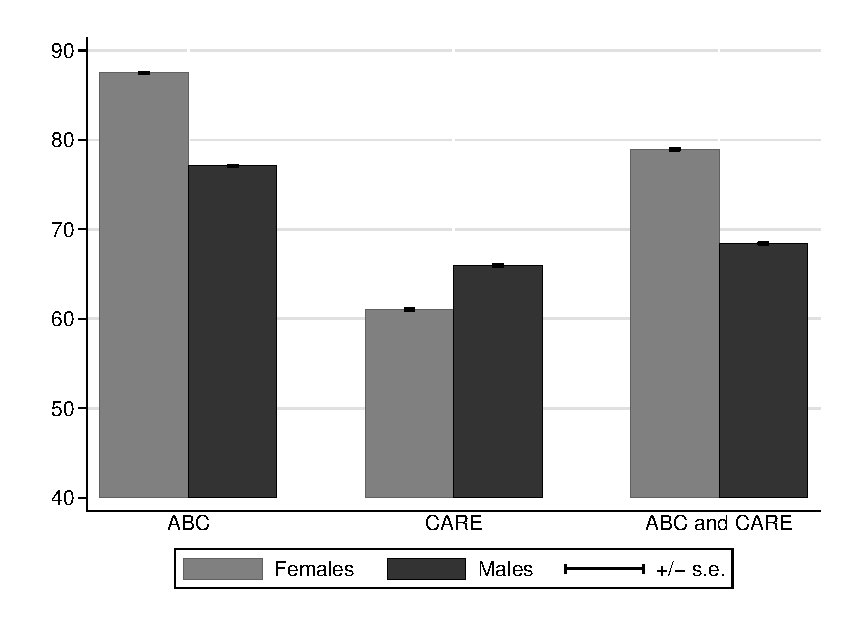
\includegraphics[width=\textwidth]{output/itt_noctrl_all.eps}
\end{subfigure}
	\begin{subfigure}[h]{0.7\textwidth}
	\centering
	\caption{Treatment vs. Next Best, Significant at 10\% Level} \label{fig:ppositive10}
		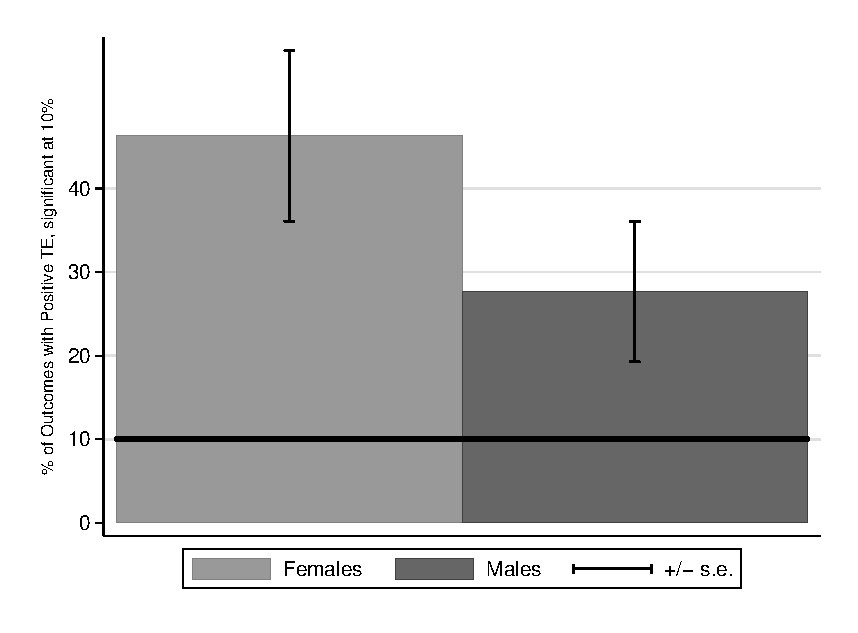
\includegraphics[width=\textwidth]{output/itt_noctrl_all_sig10.eps}
\end{subfigure}
\footnotesize \justify
Note: Panel (a) percentage of outcomes displaying a positive treatment effect, comparing treatment to next best. Panel (b) percentage of outcomes displaying a positive and statistically significant treatment effect (10\% significance level).
\end{figure}

This difference in the results depending on the counterfactual, as well as the gender differences in the treatment effects, drives our discussion of the interaction between the treatment, the family inputs, and any potential alternate center-based care. The explanation that males are more fragile than females early in life is consistent with the early differences favoring females.\footnote{\citet{Kottelenberg-Lehrer_2014_Gender-Effects,Baker_Gruber_Milligan_2015_Noncog_Defects, Schore_2017_IMHJ}.} Building on this, we explore how these early-life differences evolve for specific outcomes that are central to the analysis of  \citet{Garcia_Heckman_Leaf_etal_2017_Comp_CBA_Unpublished}, such as crime and income. We find that the treatment narrows or reverses the male-female gap for many outcomes, including education and employment. Treatment widens the male-female gap for health.

We next report estimates of the proportion of beneficial effects by outcome category and overall.\footnote{We consider a total of 95 outcomes that we classify in Appendix~\ref{appendix:results}. These are the outcomes that most clearly relate to the treatment offered by the program.} The analysis is based on treatment effect \eqref{eq:effect}. Figure~\ref{fig:ppositive} displays the results from this analysis: ABC/CARE positively impacted a large percentage of the outcomes. We show the counts for treatment compared to the next best alternative chosen by parents in Figure~\ref{fig:ppositivenb}. Proportionately more outcomes are beneficial for females, but the proportions are high for both groups and well above the benchmark of 1/2. In Tables~\ref{table:abccare_rslt_pooled_counts} to \ref{table:abccare_rslt_female_counts_n10a10} of Appendix~\ref{appendix:results}, we document a large and precisely determined fraction of beneficial treatment effects well above 1/2 for both genders for categories of outcomes spanning the life cycle through the mid 30's.

Using an $\alpha$-level of significance, one would expect to find that $\alpha\%$ of the treatment effects are ``statistically significant,'' even if the null hypothesis of no effect of the program is true simply by chance. At a 10\% level of significance, $46\%$ are statistically significant for females and $28\%$ for males (see Figure~\ref{fig:ppositive10}).

Figures~\ref{fig:ppositivehome} and Figure~\ref{fig:ppositivealternative} adjust the count in Figure~\ref{fig:ppositivenb} to analyze more clearly defined counterfactuals: treatment compared to staying at home and treatment compared to alternative preschool. These comparisons indicate that males and females benefit differently from alternatives to high quality treatment. Compared across all categories, females benefit more from treatment when compared to staying at home (as opposed to attending alternative preschools), while males benefit more from treatment when compared to attending an alternative childcare arrangement (as opposed to staying at home).

\begin{sidewaysfigure}[!htbp]
\centering
\caption{Positively Impacted Outcomes, ABC/CARE Males and Females}\label{fig:ppositive}
\begin{subfigure}[h]{0.4\textwidth}
		\centering
		\caption{Treatment vs. Next Best} \label{fig:ppositivenb}
		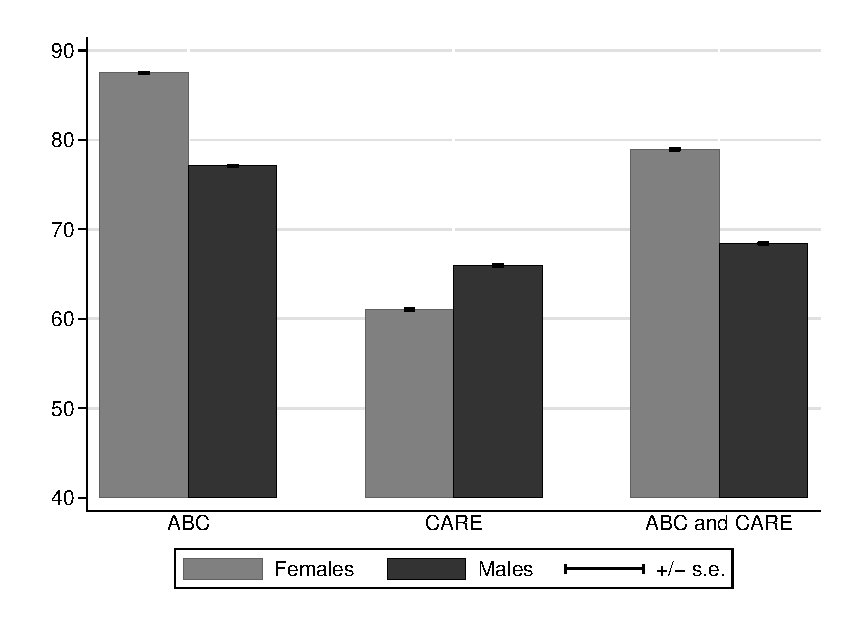
\includegraphics[width=\textwidth]{output/itt_noctrl_all.eps}
\end{subfigure}%
\begin{subfigure}[h]{0.4\textwidth}
	\centering
	\caption{Treatment vs. Next Best, Significant at 10\% Level} \label{fig:ppositive10}
		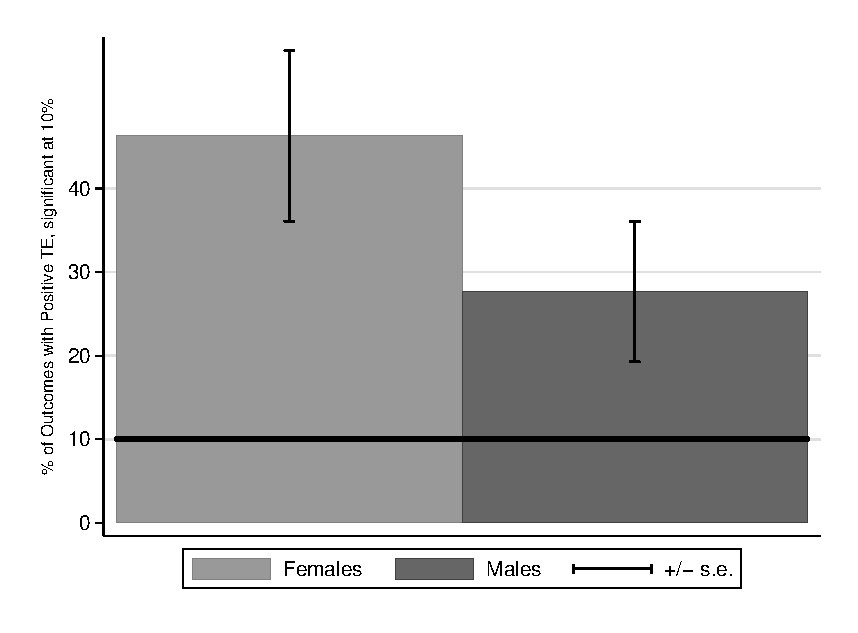
\includegraphics[width=\textwidth]{output/itt_noctrl_all_sig10.eps}
\end{subfigure}
\begin{subfigure}[h]{0.4\textwidth}
		\centering
		\caption{ Treatment vs. Stay at Home} \label{fig:ppositivehome}
		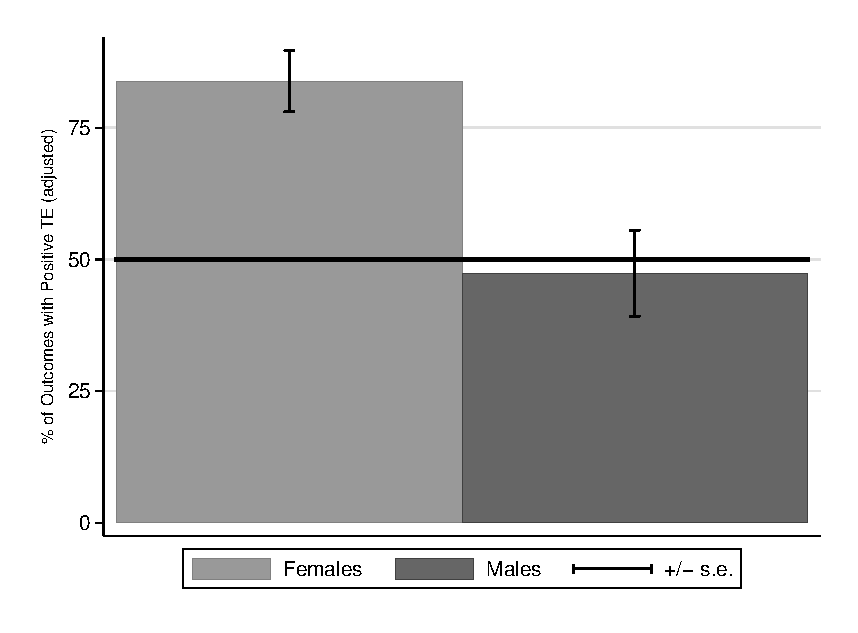
\includegraphics[width=\textwidth]{output/epan_ipw_p0_all.eps}
\end{subfigure}%
\begin{subfigure}[h]{0.4\textwidth}
	\centering
	\caption{Treatment vs. Alternative Preschool} \label{fig:ppositivealternative}
		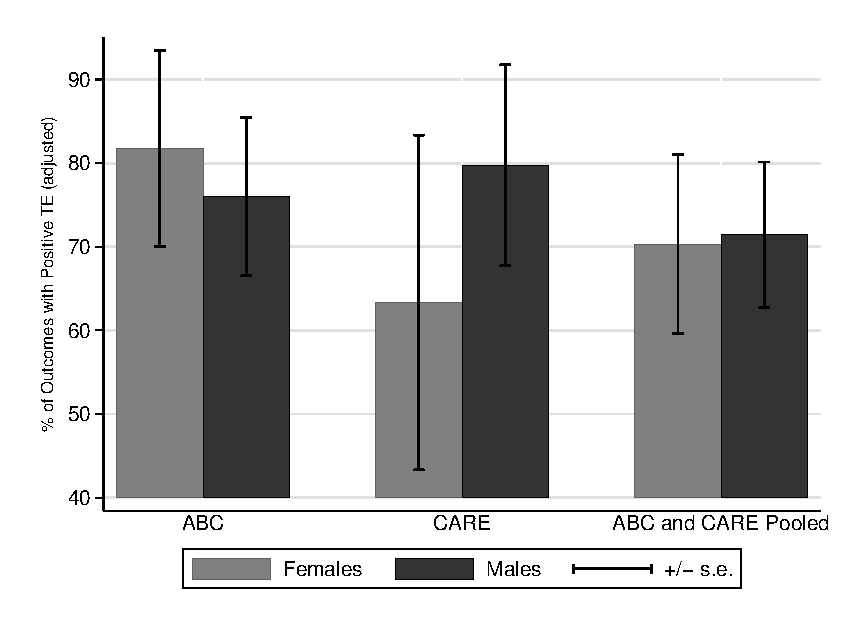
\includegraphics[width=\textwidth]{output/epan_ipw_p1_all.eps}
\end{subfigure}
\scriptsize \justify
Note: Panel (a) percentage of outcomes displaying a positive treatment effect, comparing treatment to next best. Panel (b) percentage of outcomes displaying a positive and statistically significant treatment effect (10\% significance level). Panel (c) displays the percentage of outcomes with a positive treatment effect, comparing treatment to staying at home. Panel (d) displays the percentage of outcomes with a positive treatment effect, comparing treatment to alternative childcare arrangements. Standard errors are based on the empirical bootstrap distribution. For Panel (b) we perform a ``double bootstrap'' procedure to first determine significant treatment effects at $10\%$ level and then calculate the standard error of the count.\\
\end{sidewaysfigure}

Finally, we present the estimates of the combining functions by outcome category. Figure~\ref{fig:cats-positive-significant} shows the estimated proportions that are significantly positive at the 10\% level. Consistent with the treatment effects above, control-group females tend to do better in alternative preschools than at home. This is especially true for parenting measures, IQ, education, and employment. Control-group males, on the other hand, do better at home, with more positive treatment effects in comparison to alternative preschool. The treatment effects on IQ and achievement scores, education, and employment are larger when fixing the control group to the alternative preschool.

\begin{figure}[!htbp]
\centering
\caption{Positively Impacted Outcomes by Category, ABC/CARE Males and Females}\label{fig:cats-positive-significant}
\begin{subfigure}[h]{0.7\textwidth}
	\centering
	\caption{Treatment vs. Stay at Home, Significant at 10\% Level} 
		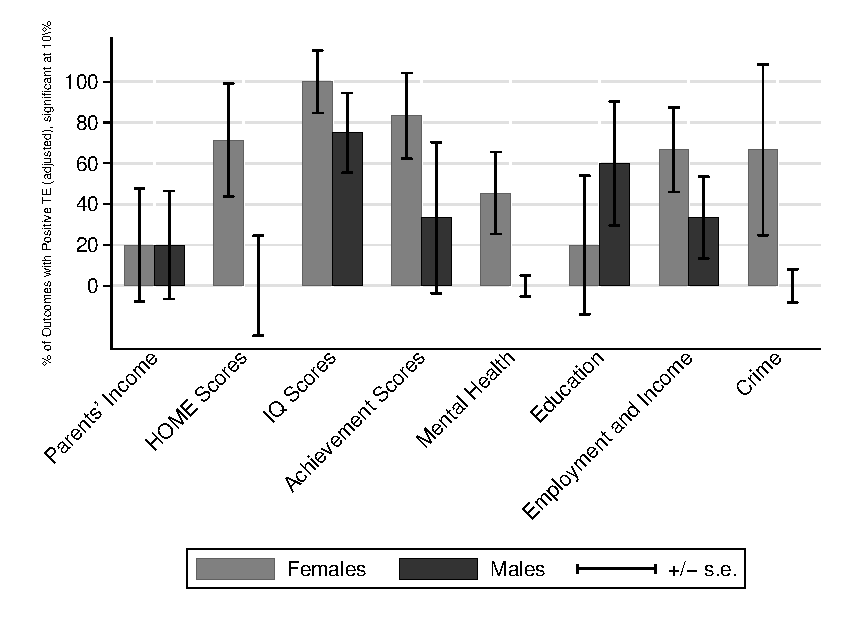
\includegraphics[width=\textwidth]{output/epan_ipw_p0_cats1_sig10.eps}
\end{subfigure}

\begin{subfigure}[h]{0.7\textwidth}
	\centering
	\caption{Treatment vs. Alternative Preschool, Significant at 10\% Level}
		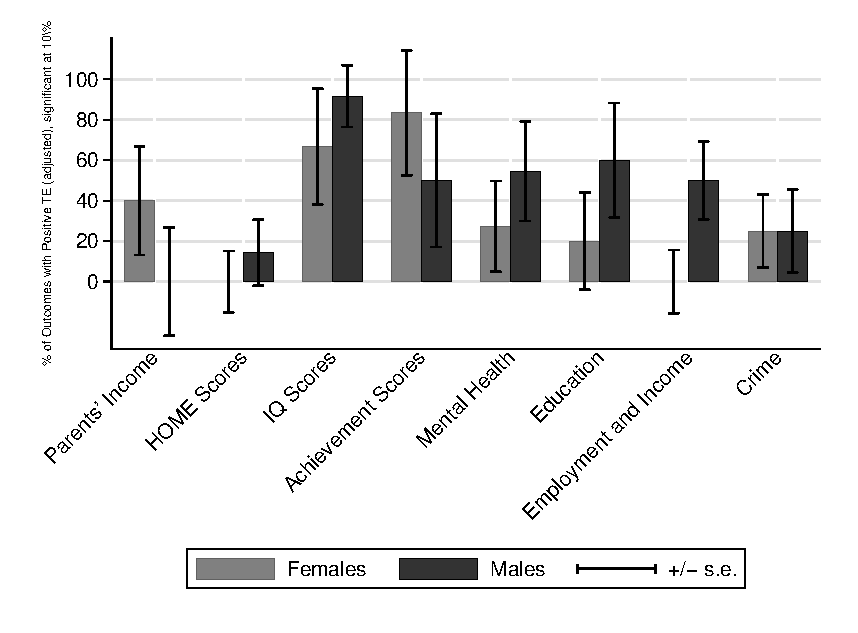
\includegraphics[width=\textwidth]{output/epan_ipw_p1_cats1_sig10.eps}
\end{subfigure}
\scriptsize \justify
Note: Panel (a) percentage of outcomes displaying a positive treatment effect, comparing treatment to next best. Panel (b) percentage of outcomes displaying a positive and statistically significant treatment effect (10\% significance level). Panel (c) displays the percentage of outcomes with a positive treatment effect, comparing treatment to staying at home. Panel (d) displays the percentage of outcomes with a positive treatment effect, comparing treatment to alternative childcare arrangements. Standard errors are based on the empirical bootstrap distribution. For Panel (b) we perform a ``double bootstrap'' procedure to first determine significant treatment effects at $10\%$ level and then calculate the standard error of the count.\\
\end{figure}

\textbf{[JJH: Report estimates here.]}

\section{Gender Differences}
\label{sec:gender-differences}
\subsection{Possible Explanations for Gender Differences}

\textbf{[JJH: Way too much emphasis on CBA.]}

These results and estimates of IRR/CBA \citep{Garcia_Heckman_Leaf_etal_2017_Comp_CBA_Unpublished} show gender differences. In this section, we discuss some of the mechanisms contributing to these differences and connect the results of the two papers.

On a superficial level, there is tension between the results in this paper favoring females and the results in \citet{Garcia_Heckman_Leaf_etal_2017_Comp_CBA_Unpublished} favoring males. There are two mutually inclusive explanations for this. One explanation is that although a larger proportion of the treatment effects are positive for females, those that are positive for males correspond to outcomes that can be monetized. For example, there is a strong treatment effect on labor income at age 30 for males, but not for females. When this income is projected over the life cycle in \citet{Garcia_Heckman_Leaf_etal_2017_Comp_CBA_Unpublished}, the males continue to benefit more from treatment than do females. In a related case, there are also outcomes that cannot be monetized for which treatment more positively impacts for females than for males. An example of this are variables related to family structure, such as number of children.

Another explanation for the higher benefit/cost ratio and internal rate of return for males is that even if there are treatment effects for both genders, a general characteristic of males in society can change the expression of that effect. An example of this is seen in crime. ABC/CARE positively and significantly reduced crime for both males and females. However, on average, males commit more crimes that have higher social costs (e.g. violent crimes) compared with females. Figure~\ref{fig:crime-tes-detail} illustrates this. Although ABC/CARE reduces criminal activity both of misdemeanors and felonies, the mean number of misdemeanors committed by the control-group females is very close to the analogous mean of the control-group males. This is not the case for felonies, which tend to be more serious (and costly) crimes.\footnote{This is also supported by \citet{Cohen-Bowles_2010_Estimating-Cost-Crime,Gregg_etal_2015_SocialRealities_BOOK,UDOJ_2016_PrisonersStatistics_Bulletin}.}

\begin{figure}[!htbp]
\centering
\caption{Treatment Effects on Crime, by Crime Type}
\label{fig:crime-tes-detail}
\begin{subfigure}[h]{0.5\textwidth}
	\centering
	\caption{Misdemeanors}
	\label{fig:crime-misdemeanors}
	\includegraphics[width=\textwidth]{output/bar-gender-trt-ad34_mis}
\end{subfigure}%
\begin{subfigure}[h]{0.5\textwidth}
	\centering
	\caption{Felonies}
	\label{fig:crime-felonies}
	\includegraphics[width=\textwidth]{output/bar-gender-trt-ad34_fel}
\end{subfigure}
\footnotesize \justify
Note: These plots show the mean misdemeanors and felonies of the treatment and control group by gender. The capped lines indicate standard errors and the points represent significant differences between treatment and control within each gender. These are estimated using 100 bootstraps. Both of these measures come from the administrative crime data collected when the subjects were approximately age 35.
\end{figure}

There is another important factor at play that is present in the results of both papers: the issue of alternative preschool. There are substantial differences between males and females in one counterfactual: treatment vs. alternative preschools. The estimated treatment effects are very similar across genders for treatment compared to those staying at home full time. Males benefit much more from treatment relative to alternative preschools compared to their benefits from treatment relative to staying at home. This result is consistent with findings noted elsewhere: (i) stark gender differences resulting from attending low quality childcare \citep{Kottelenberg-Lehrer_2014_Gender-Effects,Baker_Gruber_Milligan_2015_Noncog_Defects}; and (ii) females are less sensitive to uncertain environments (see, e.g., \citealp{Autor-etal_2015_Family-Disadvantage}).

In addition to a gender difference in alternative preschool experiences, there are gender differences in the experience of ABC/CARE treatment. We explore this by looking at the specific effects of the intervention on parenting.\footnote{In this exercise, we use We use measurements of the Home Observation for Measurement of the Environment (HOME; \citet{Bradley-Caldwell_1977_AJMD}). Although the exact scales vary by age, the subscales of the HOME measure generally measure maternal warmth and involvement, absence of punishment, provision of appropriate toys, encouragement of mature behavior and independence, and the physical and language environment. The full score is the sum of these subscales.}

When graphing the density of a factor combining the parenting skills measured at different ages, the density of the treatment group in both the male and female subsamples is bimodal (Figure~\ref{fig:total-home}). Because this is not the case for the control group, it is possible that treatment is moderated by another input of home environment. We consider the input of father's presence because it is highly correlated with selection into alternative preschool. For males, the mean of the treatment group if the father is present is greater than that of the treatment group if the father is absent. The reverse is seen for the females.

\begin{figure}
\begin{center}
\caption{Density of the HOME Scores by Gender and Experimental Group}
\label{fig:total-home}

	\begin{subfigure}[b]{0.49\textwidth}
		\centering
		\caption{Parenting Skills, Males}
		\label{fig:home-male-factor}
			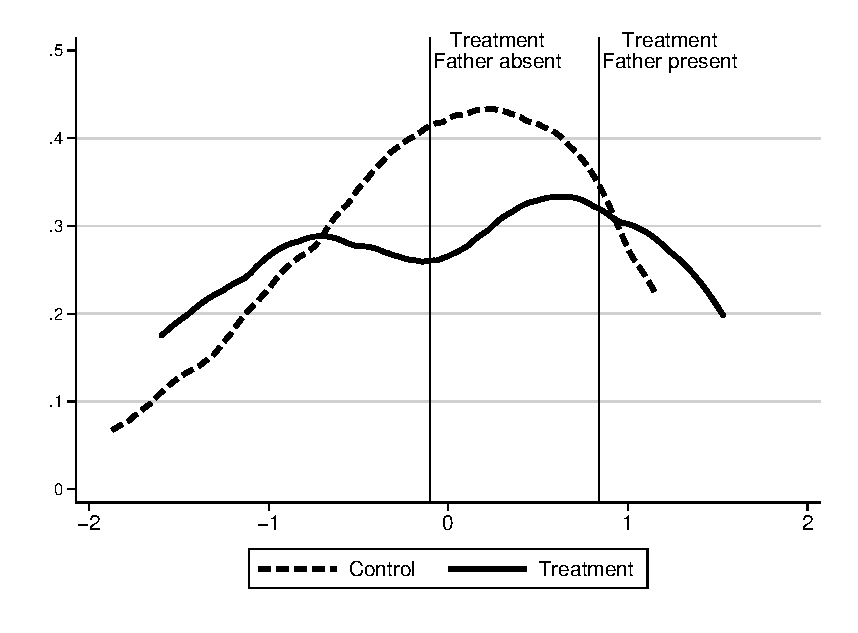
\includegraphics[width=\textwidth]{output/HOME-males-factorhome}
	\end{subfigure}
	\begin{subfigure}[b]{0.49\textwidth}
		\centering
		\caption{Parenting Skills, Females}
		\label{fig:home-female-factor}
			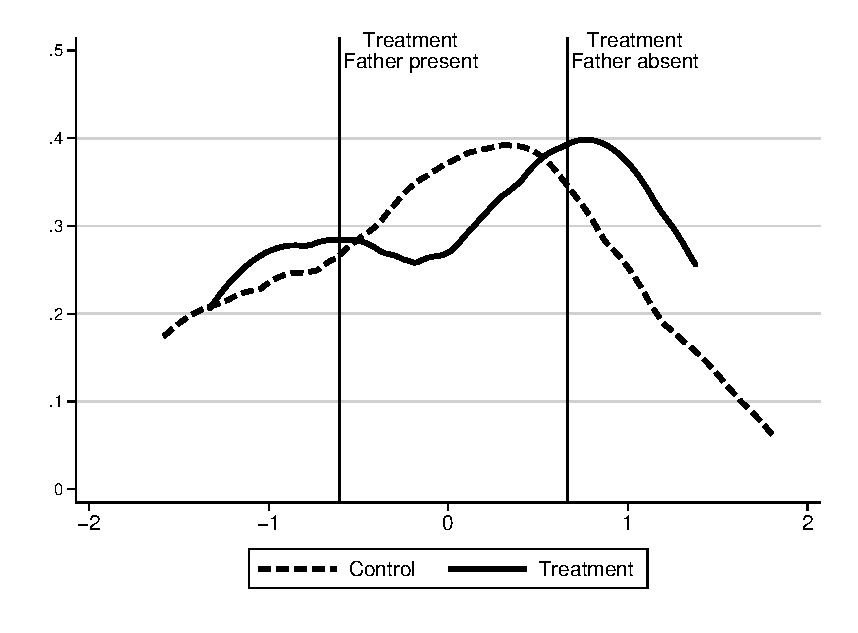
\includegraphics[width=\textwidth]{output/HOME-females-factorhome}
	\end{subfigure}
\end{center}
\raggedright
Note: These plots show the distribution the factor of HOME scores. The factors are computed by gender using full HOME scores at 0.5, 1.5, 2.5, and 8 years. The vertical lines are the means of the treatment group by father's presence.
\end{figure}

We explore this trend more closely in Figure~\ref{fig:total-home-quantiles}. To do so, we calculate the distribution pooling experimental groups but splitting by gender and father's presence. We then calculate, by gender and father's presence, the proportion of the treatment group that is in quantile 1 versus quantile 2. We do the same for the control group.

\begin{sidewaysfigure}
\begin{center}
\caption{Factor HOME Scores}
\label{fig:total-home-quantiles}
	\begin{subfigure}[b]{0.49\textwidth}
		\centering
		\caption{HOME, Father Absent, Males}
		\label{fig:home-male-mean}
			\includegraphics[width=\textwidth]{output/HOME-male1-fhome0-2quant}
	\end{subfigure}
	\begin{subfigure}[b]{0.49\textwidth}
		\centering
		\caption{HOME, Father Absent, Females}
		\label{fig:home-female-mean}
			\includegraphics[width=\textwidth]{output/HOME-male0-fhome0-2quant}
	\end{subfigure}
	
	\begin{subfigure}[b]{0.49\textwidth}
		\centering
		\caption{HOME, Father Present, Males}
		\label{fig:home-male-factor}
			\includegraphics[width=\textwidth]{output/HOME-male1-fhome1-2quant}
	\end{subfigure}
	\begin{subfigure}[b]{0.49\textwidth}
		\centering
		\caption{HOME, Father Present, Females}
		\label{fig:home-female-factor}
			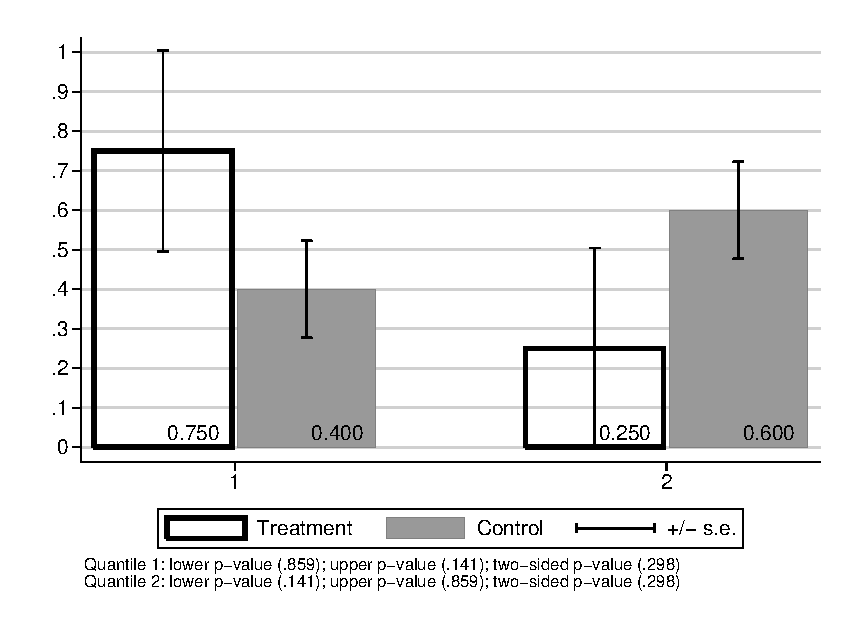
\includegraphics[width=\textwidth]{output/HOME-male0-fhome1-2quant}
	\end{subfigure}
\end{center}
\raggedright \footnotesize
Note: The horizontal axis divides a factor of the HOME scores into the first and second quantile of the distribution pooling across experimental groups, but splitting  by gender and father's presence. The factors are computed by gender using full HOME scores at 0.5, 1.5, 2.5, and 8 years. The lower $p$-value tests that the treatment proportion is less than the control proportion within a quantile. The upper $p$-value tests that the treatment proportion is greater than the control proportion within a quantile. The numbers reported in the bars are the proportions. All standard errors and $p$-values are calculated using 1,000 bootstraps.
\end{sidewaysfigure}

The result of this exercise shows that the bimodal shape of the densities of the treatment group is explained differently by gender. For males, the parenting measures are higher for the control group when the fathers are absent and higher for the treatment group when father's are present. For females, the opposite is the case: The parenting measures are higher for the control group when fathers are present and higher for the treatment group when fathers are absent.

This example illustrates that treatment complements father's presence for males but substitutes it for females. That is, treatment compensates for early life disadvantage for males, but substitutes it for females. This explains how early-life skill differences favoring females can still translate to later-life outcomes favoring males. Although males initially face deficits, the program compensates for these deficits helping them catch up to females. Additional factors in the larger economy can then widen differences later in life when the subjects enter the labor market.

\textbf{[JJH: Report results for controls (see comment 7a \& 7b). We need to deemphasize CBA. We are spoiling its market.]}




\section{Conclusion}
\label{sec:conclusion}
\textbf{[JJH: Need to point out consistency with the literature.][We edited the conclusion to connect more with the literature.]}

Although several studies of early childhood education report effects by gender, they do not consider two important factors. The first factor is that there can be gender gaps before treatment that are then changed after treatment. We find that control-group males tend to do better than the control-group females, especially in education and employment outcomes. After treatment, most these gaps are narrowed or reversed. This corresponds with the finding that a larger proportion of the treatment effects are positive and significant for females than for males. ABC/CARE, in addition to improving select individual outcomes, also narrowed the male-female gap in important categories of outcomes. 

The second factor to consider is the alternative setting. We find that lower quality preschools are especially detrimental for boys. This connects to previous work that finds boys to be more vulnerable early in life than girls \citep{golding2016psychology}. Boys similarly are more harmed by unstable home environments (measured by father present and maternal locus of control) than girls. 



\clearpage
\singlespacing
\bibliography{../heckman}
\bibliographystyle{chicago}

\end{document}
